%% bm.pdf preamble - material merged from previous preamble and current pandoc preamable output
% NOTE: float placement required changes to the source files referenced by bm.tex
% May 28, 2020
%
% Use lualatex to compile - test with MiKTeX 2.9

% uncomment to list all files in log
%\listfiles

\documentclass[12pt]{report}


\usepackage{fontspec}

%\setmainfont[Scale=MatchLowercase]{Lucida Bright}
%\setmonofont{FreeMono}
%\setmonofont{Source Code Pro}
\setmonofont[Scale=MatchLowercase]{Ubuntu Mono}

% short snippets of asian languages
\newfontfamily\myAsian{Noto Serif TC Medium}

\usepackage[headings]{fullpage}

% national use characters 
%\usepackage{inputenc}

% ams mathematical symbols
\usepackage{amsmath,amssymb}

% added to support pandoc highlighting
\usepackage{microtype}

\usepackage{makeidx}

% add index and bibliographies to table of contents
\usepackage[nottoc]{tocbibind}

% postscript courier and times in place of cm fonts
%\usepackage{courier}
%\usepackage{times}

% extended coloring
\usepackage{color}
\usepackage[table,dvipsnames]{xcolor}
\usepackage{colortbl}

% advanced date formating
\usepackage{datetime}

%support pandoc code highlighting
\usepackage{fancyvrb}

% \DefineShortVerb[commandchars=\\\{\}]{\|}
% \DefineVerbatimEnvironment{Highlighting}{Verbatim}{commandchars=\\\{\}}
% % Add ',fontsize=\small' for more characters per line

% tango style colors
% \usepackage{framed}
% \definecolor{shadecolor}{RGB}{255,255,255}
% \newenvironment{Shaded}{\begin{snugshade}}{\end{snugshade}}
% \newcommand{\KeywordTok}[1]{\textcolor[rgb]{0.13,0.29,0.53}{\textbf{{#1}}}}
% \newcommand{\DataTypeTok}[1]{\textcolor[rgb]{0.13,0.29,0.53}{{#1}}}
% \newcommand{\DecValTok}[1]{\textcolor[rgb]{0.00,0.00,0.81}{{#1}}}
% \newcommand{\BaseNTok}[1]{\textcolor[rgb]{0.00,0.00,0.81}{{#1}}}
% \newcommand{\FloatTok}[1]{\textcolor[rgb]{0.00,0.00,0.81}{{#1}}}
% \newcommand{\CharTok}[1]{\textcolor[rgb]{0.31,0.60,0.02}{{#1}}}
% \newcommand{\StringTok}[1]{\textcolor[rgb]{0.31,0.60,0.02}{{#1}}}
% \newcommand{\CommentTok}[1]{\textcolor[rgb]{0.56,0.35,0.01}{\textit{{#1}}}}
% \newcommand{\OtherTok}[1]{\textcolor[rgb]{0.56,0.35,0.01}{{#1}}}
% \newcommand{\AlertTok}[1]{\textcolor[rgb]{0.94,0.16,0.16}{{#1}}}
% \newcommand{\FunctionTok}[1]{\textcolor[rgb]{0.00,0.00,0.00}{{#1}}}
% \newcommand{\RegionMarkerTok}[1]{{#1}}
% \newcommand{\ErrorTok}[1]{\textbf{{#1}}}
% \newcommand{\NormalTok}[1]{{#1}}

% %espresso style colors
% \usepackage{framed}
% \definecolor{shadecolor}{RGB}{42,33,28}
% \newenvironment{Shaded}{\begin{snugshade}}{\end{snugshade}}
% \newcommand{\KeywordTok}[1]{\textcolor[rgb]{0.26,0.66,0.93}{\textbf{{#1}}}}
% \newcommand{\DataTypeTok}[1]{\textcolor[rgb]{0.74,0.68,0.62}{\underline{{#1}}}}
% \newcommand{\DecValTok}[1]{\textcolor[rgb]{0.27,0.67,0.26}{{#1}}}
% \newcommand{\BaseNTok}[1]{\textcolor[rgb]{0.27,0.67,0.26}{{#1}}}
% \newcommand{\FloatTok}[1]{\textcolor[rgb]{0.27,0.67,0.26}{{#1}}}
% \newcommand{\CharTok}[1]{\textcolor[rgb]{0.02,0.61,0.04}{{#1}}}
% \newcommand{\StringTok}[1]{\textcolor[rgb]{0.02,0.61,0.04}{{#1}}}
% \newcommand{\CommentTok}[1]{\textcolor[rgb]{0.00,0.40,1.00}{\textit{{#1}}}}
% \newcommand{\OtherTok}[1]{\textcolor[rgb]{0.74,0.68,0.62}{{#1}}}
% \newcommand{\AlertTok}[1]{\textcolor[rgb]{1.00,1.00,0.00}{{#1}}}
% \newcommand{\FunctionTok}[1]{\textcolor[rgb]{1.00,0.58,0.35}{\textbf{{#1}}}}
% \newcommand{\RegionMarkerTok}[1]{\textcolor[rgb]{0.74,0.68,0.62}{{#1}}}
% \newcommand{\ErrorTok}[1]{\textcolor[rgb]{0.74,0.68,0.62}{\textbf{{#1}}}}
% \newcommand{\NormalTok}[1]{\textcolor[rgb]{0.74,0.68,0.62}{{#1}}}

% %kete style colors
% \newenvironment{Shaded}{}{}
% \newcommand{\KeywordTok}[1]{\textbf{{#1}}}
% \newcommand{\DataTypeTok}[1]{\textcolor[rgb]{0.50,0.00,0.00}{{#1}}}
% \newcommand{\DecValTok}[1]{\textcolor[rgb]{0.00,0.00,1.00}{{#1}}}
% \newcommand{\BaseNTok}[1]{\textcolor[rgb]{0.00,0.00,1.00}{{#1}}}
% \newcommand{\FloatTok}[1]{\textcolor[rgb]{0.50,0.00,0.50}{{#1}}}
% \newcommand{\CharTok}[1]{\textcolor[rgb]{1.00,0.00,1.00}{{#1}}}
% \newcommand{\StringTok}[1]{\textcolor[rgb]{0.87,0.00,0.00}{{#1}}}
% \newcommand{\CommentTok}[1]{\textcolor[rgb]{0.50,0.50,0.50}{\textit{{#1}}}}
% \newcommand{\OtherTok}[1]{{#1}}
% \newcommand{\AlertTok}[1]{\textcolor[rgb]{0.00,1.00,0.00}{\textbf{{#1}}}}
% \newcommand{\FunctionTok}[1]{\textcolor[rgb]{0.00,0.00,0.50}{{#1}}}
% \newcommand{\RegionMarkerTok}[1]{{#1}}
% \newcommand{\ErrorTok}[1]{\textcolor[rgb]{1.00,0.00,0.00}{\textbf{{#1}}}}
% \newcommand{\NormalTok}[1]{{#1}}
% %end pandoc code hacks

% jodliterate colors
\usepackage{color}
\definecolor{shadecolor}{RGB}{248,248,248}
% j control structures 
\definecolor{keywcolor}{rgb}{0.13,0.29,0.53}
% j explicit arguments x y m n u v
\definecolor{datacolor}{rgb}{0.13,0.29,0.53}
% j numbers - all types see j.xml
\definecolor{decvcolor}{rgb}{0.00,0.00,0.81}
\definecolor{basencolor}{rgb}{0.00,0.00,0.81}
\definecolor{floatcolor}{rgb}{0.00,0.00,0.81}
% j local assignments
\definecolor{charcolor}{rgb}{0.31,0.60,0.02}
\definecolor{stringcolor}{rgb}{0.31,0.60,0.02}
\definecolor{commentcolor}{rgb}{0.56,0.35,0.01}
% primitive adverbs and conjunctions
%\definecolor{othercolor}{rgb}{0.56,0.35,0.01}   
\definecolor{othercolor}{RGB}{0,0,255}
% global assignments
\definecolor{alertcolor}{rgb}{0.94,0.16,0.16}
% primitive J verbs and noun names
\definecolor{funccolor}{rgb}{0.00,0.00,0.00}

% custom colors
\definecolor{CodeBackGround}{cmyk}{0.0,0.0,0,0.05}    % light gray
\definecolor{CodeComment}{rgb}{0,0.50,0.00}           % dark green {0,0.45,0.08}
\definecolor{TableStripes}{gray}{0.9}                 % odd/even background in tables

% Colors for the hyperref package
\definecolor{urlcolor}{rgb}{0,.145,.698}
\definecolor{linkcolor}{rgb}{.71,0.21,0.01}
\definecolor{citecolor}{rgb}{.12,.54,.11}

% % Exact colors from NB
\definecolor{incolor}{HTML}{303F9F}
\definecolor{outcolor}{HTML}{D84315}
\definecolor{cellborder}{HTML}{CFCFCF}
\definecolor{cellbackground}{HTML}{F7F7F7}

% % ANSI colors
\definecolor{ansi-black}{HTML}{3E424D}
\definecolor{ansi-black-intense}{HTML}{282C36}
\definecolor{ansi-red}{HTML}{E75C58}
\definecolor{ansi-red-intense}{HTML}{B22B31}
\definecolor{ansi-green}{HTML}{00A250}
\definecolor{ansi-green-intense}{HTML}{007427}
\definecolor{ansi-yellow}{HTML}{DDB62B}
\definecolor{ansi-yellow-intense}{HTML}{B27D12}
\definecolor{ansi-blue}{HTML}{208FFB}
\definecolor{ansi-blue-intense}{HTML}{0065CA}
\definecolor{ansi-magenta}{HTML}{D160C4}
\definecolor{ansi-magenta-intense}{HTML}{A03196}
\definecolor{ansi-cyan}{HTML}{60C6C8}
\definecolor{ansi-cyan-intense}{HTML}{258F8F}
\definecolor{ansi-white}{HTML}{C5C1B4}
\definecolor{ansi-white-intense}{HTML}{A1A6B2}
\definecolor{ansi-default-inverse-fg}{HTML}{FFFFFF}
\definecolor{ansi-default-inverse-bg}{HTML}{000000}
    

% \usepackage{framed}
% \newenvironment{Shaded}{}{}
% \newcommand{\KeywordTok}[1]{\textcolor{keywcolor}{\textbf{{#1}}}}
% \newcommand{\DataTypeTok}[1]{\textcolor{datacolor}{{#1}}}
% %\newcommand{\DecValTok}[1]{\textcolor{decvcolor}{{#1}}}
% \newcommand{\DecValTok}[1]{{#1}} 
% \newcommand{\BaseNTok}[1]{\textcolor{basencolor}{{#1}}}
% \newcommand{\FloatTok}[1]{\textcolor{floatcolor}{{#1}}}
% \newcommand{\CharTok}[1]{\textcolor{charcolor}{\textbf{{#1}}}}
% \newcommand{\StringTok}[1]{\textcolor{stringcolor}{{#1}}}
% \newcommand{\CommentTok}[1]{\textcolor{commentcolor}{\textit{{#1}}}}
% \newcommand{\OtherTok}[1]{\textcolor{othercolor}{{#1}}} 
% \newcommand{\AlertTok}[1]{\textcolor{alertcolor}{\textbf{{#1}}}}
% %\newcommand{\FunctionTok}[1]{\textcolor{funccolor}{{#1}}}
% \newcommand{\FunctionTok}[1]{{#1}}
% \newcommand{\RegionMarkerTok}[1]{{#1}}
% \newcommand{\ErrorTok}[1]{\textbf{{#1}}}
% \newcommand{\NormalTok}[1]{{#1}}

% The default LaTeX title has an obnoxious amount of whitespace. By default,
% titling removes some of it. It also provides customization options.
\usepackage{titling}

% headers and footers
\usepackage{fancyhdr}
%\pagestyle{fancy}
\pagestyle{plain}

\fancyhead{}
\fancyfoot{}

%\fancyhead[LE,RO]{\slshape \rightmark}
%\fancyhead[LO,RE]{\slshape \leftmark}
\fancyfoot[C]{\thepage}
%\headrulewidth 0.4pt
%\footrulewidth 0 pt

%\addtolength{\headheight}{\baselineskip}

%\lfoot{\emph{Analyze the Data not the Drivel}}
%\rfoot{\emph{\today}}

% subfigure handles figures that contain subfigures
%\usepackage{color,graphicx,subfigure,sidecap}
\usepackage{graphicx,sidecap}
\usepackage{subfigure}
\graphicspath{{./inclusions/}}

% floatflt provides for text wrapping around small figures and tables
\usepackage{floatflt}

% tweak caption formats 
\usepackage{caption} 
\usepackage{sidecap}
%\usepackage{subcaption} % not compatible with subfigure

\usepackage{rotating} % flip tables sideways

% complex footnotes
%\usepackage{bigfoot}

% weird logos \XeLaTeX
\usepackage{metalogo}

\newcommand{\HRule}{\rule{\linewidth}{0.5mm}}

\usepackage[breakable]{tcolorbox}

\usepackage{parskip} % Stop auto-indenting (to mimic markdown behaviour)
    
% Basic figure setup, for now with no caption control since it's done
% automatically by Pandoc (which extracts ![](path) syntax from Markdown).
\usepackage{graphicx}

%\DeclareCaptionFormat{nocaption}{}
%\captionsetup{format=nocaption,aboveskip=0pt,belowskip=0pt}

\usepackage[Export]{adjustbox} % Used to constrain images to a maximum size
\adjustboxset{max size={0.9\linewidth}{0.9\paperheight}}
\usepackage{float}

%\floatplacement{figure}{H} % forces figures to be placed at the correct location

\usepackage{xcolor} % Allow colors to be defined
\usepackage{enumerate} % Needed for markdown enumerations to work
\usepackage{geometry} % Used to adjust the document margins

%\usepackage{amsmath} % Equations
%\usepackage{amssymb} % Equations

\usepackage{textcomp} % defines textquotesingle

% Hack from http://tex.stackexchange.com/a/47451/13684:
\AtBeginDocument{%
	\def\PYZsq{\textquotesingle}% Upright quotes in Pygmentized code
}

\usepackage{upquote} % Upright quotes for verbatim code
\usepackage{eurosym} % defines \euro
\usepackage[mathletters]{ucs} % Extended unicode (utf-8) support

%\usepackage{fancyvrb} % verbatim replacement that allows latex

\usepackage{grffile} % extends the file name processing of package graphics 
					 % to support a larger range
					 
\makeatletter % fix for grffile with XeLaTeX
\def\Gread@@xetex#1{%
  \IfFileExists{"\Gin@base".bb}%
  {\Gread@eps{\Gin@base.bb}}%
  {\Gread@@xetex@aux#1}%
}
\makeatother

% The hyperref package gives us a pdf with properly built
% internal navigation ('pdf bookmarks' for the table of contents,
% internal cross-reference links, web links for URLs, etc.)
\usepackage{hyperref}
% The default LaTeX title has an obnoxious amount of whitespace. By default,
% titling removes some of it. It also provides customization options.
\usepackage{titling}
\usepackage{longtable} % longtable support required by pandoc >1.10
\usepackage{booktabs}  % table support for pandoc > 1.12.2
\usepackage[inline]{enumitem} % IRkernel/repr support (it uses the enumerate* environment)
\usepackage[normalem]{ulem} % ulem is needed to support strikethroughs (\sout)
							% normalem makes italics be italics, not underlines
\usepackage{mathrsfs}

% commands and environments needed by pandoc snippets
% extracted from the output of `pandoc -s`
\providecommand{\tightlist}{%
  \setlength{\itemsep}{0pt}\setlength{\parskip}{0pt}}
  
\DefineVerbatimEnvironment{Highlighting}{Verbatim}{commandchars=\\\{\}}
% Add ',fontsize=\small' for more characters per line
\newenvironment{Shaded}{}{}
\newcommand{\KeywordTok}[1]{\textcolor[rgb]{0.00,0.44,0.13}{\textbf{{#1}}}}
\newcommand{\DataTypeTok}[1]{\textcolor[rgb]{0.56,0.13,0.00}{{#1}}}
\newcommand{\DecValTok}[1]{\textcolor[rgb]{0.25,0.63,0.44}{{#1}}}
\newcommand{\BaseNTok}[1]{\textcolor[rgb]{0.25,0.63,0.44}{{#1}}}
\newcommand{\FloatTok}[1]{\textcolor[rgb]{0.25,0.63,0.44}{{#1}}}
\newcommand{\CharTok}[1]{\textcolor[rgb]{0.25,0.44,0.63}{{#1}}}
\newcommand{\StringTok}[1]{\textcolor[rgb]{0.25,0.44,0.63}{{#1}}}
\newcommand{\CommentTok}[1]{\textcolor[rgb]{0.38,0.63,0.69}{\textit{{#1}}}}
\newcommand{\OtherTok}[1]{\textcolor[rgb]{0.00,0.44,0.13}{{#1}}}
\newcommand{\AlertTok}[1]{\textcolor[rgb]{1.00,0.00,0.00}{\textbf{{#1}}}}
\newcommand{\FunctionTok}[1]{\textcolor[rgb]{0.02,0.16,0.49}{{#1}}}
\newcommand{\RegionMarkerTok}[1]{{#1}}
\newcommand{\ErrorTok}[1]{\textcolor[rgb]{1.00,0.00,0.00}{\textbf{{#1}}}}
\newcommand{\NormalTok}[1]{{#1}}

% Additional commands for more recent versions of Pandoc
\newcommand{\ConstantTok}[1]{\textcolor[rgb]{0.53,0.00,0.00}{{#1}}}
\newcommand{\SpecialCharTok}[1]{\textcolor[rgb]{0.25,0.44,0.63}{{#1}}}
\newcommand{\VerbatimStringTok}[1]{\textcolor[rgb]{0.25,0.44,0.63}{{#1}}}
\newcommand{\SpecialStringTok}[1]{\textcolor[rgb]{0.73,0.40,0.53}{{#1}}}
\newcommand{\ImportTok}[1]{{#1}}
\newcommand{\DocumentationTok}[1]{\textcolor[rgb]{0.73,0.13,0.13}{\textit{{#1}}}}
\newcommand{\AnnotationTok}[1]{\textcolor[rgb]{0.38,0.63,0.69}{\textbf{\textit{{#1}}}}}
\newcommand{\CommentVarTok}[1]{\textcolor[rgb]{0.38,0.63,0.69}{\textbf{\textit{{#1}}}}}
\newcommand{\VariableTok}[1]{\textcolor[rgb]{0.10,0.09,0.49}{{#1}}}
\newcommand{\ControlFlowTok}[1]{\textcolor[rgb]{0.00,0.44,0.13}{\textbf{{#1}}}}
\newcommand{\OperatorTok}[1]{\textcolor[rgb]{0.40,0.40,0.40}{{#1}}}
\newcommand{\BuiltInTok}[1]{{#1}}
\newcommand{\ExtensionTok}[1]{{#1}}
\newcommand{\PreprocessorTok}[1]{\textcolor[rgb]{0.74,0.48,0.00}{{#1}}}
\newcommand{\AttributeTok}[1]{\textcolor[rgb]{0.49,0.56,0.16}{{#1}}}
\newcommand{\InformationTok}[1]{\textcolor[rgb]{0.38,0.63,0.69}{\textbf{\textit{{#1}}}}}
\newcommand{\WarningTok}[1]{\textcolor[rgb]{0.38,0.63,0.69}{\textbf{\textit{{#1}}}}}

% Define a nice break command that doesn't care if a line doesn't already exist.
\def\br{\hspace*{\fill} \\* }
% Math Jax compatibility definitions
\def\gt{>}
\def\lt{<}
\let\Oldtex\TeX
\let\Oldlatex\LaTeX
\renewcommand{\TeX}{\textrm{\Oldtex}}
\renewcommand{\LaTeX}{\textrm{\Oldlatex}}
 
% Pygments definitions
\makeatletter
\def\PY@reset{\let\PY@it=\relax \let\PY@bf=\relax%
    \let\PY@ul=\relax \let\PY@tc=\relax%
    \let\PY@bc=\relax \let\PY@ff=\relax}
\def\PY@tok#1{\csname PY@tok@#1\endcsname}
\def\PY@toks#1+{\ifx\relax#1\empty\else%
    \PY@tok{#1}\expandafter\PY@toks\fi}
\def\PY@do#1{\PY@bc{\PY@tc{\PY@ul{%
    \PY@it{\PY@bf{\PY@ff{#1}}}}}}}
\def\PY#1#2{\PY@reset\PY@toks#1+\relax+\PY@do{#2}}

\expandafter\def\csname PY@tok@w\endcsname{\def\PY@tc##1{\textcolor[rgb]{0.73,0.73,0.73}{##1}}}
\expandafter\def\csname PY@tok@c\endcsname{\let\PY@it=\textit\def\PY@tc##1{\textcolor[rgb]{0.25,0.50,0.50}{##1}}}
\expandafter\def\csname PY@tok@cp\endcsname{\def\PY@tc##1{\textcolor[rgb]{0.74,0.48,0.00}{##1}}}
\expandafter\def\csname PY@tok@k\endcsname{\let\PY@bf=\textbf\def\PY@tc##1{\textcolor[rgb]{0.00,0.50,0.00}{##1}}}
\expandafter\def\csname PY@tok@kp\endcsname{\def\PY@tc##1{\textcolor[rgb]{0.00,0.50,0.00}{##1}}}
\expandafter\def\csname PY@tok@kt\endcsname{\def\PY@tc##1{\textcolor[rgb]{0.69,0.00,0.25}{##1}}}
\expandafter\def\csname PY@tok@o\endcsname{\def\PY@tc##1{\textcolor[rgb]{0.40,0.40,0.40}{##1}}}
\expandafter\def\csname PY@tok@ow\endcsname{\let\PY@bf=\textbf\def\PY@tc##1{\textcolor[rgb]{0.67,0.13,1.00}{##1}}}
\expandafter\def\csname PY@tok@nb\endcsname{\def\PY@tc##1{\textcolor[rgb]{0.00,0.50,0.00}{##1}}}
\expandafter\def\csname PY@tok@nf\endcsname{\def\PY@tc##1{\textcolor[rgb]{0.00,0.00,1.00}{##1}}}
\expandafter\def\csname PY@tok@nc\endcsname{\let\PY@bf=\textbf\def\PY@tc##1{\textcolor[rgb]{0.00,0.00,1.00}{##1}}}
\expandafter\def\csname PY@tok@nn\endcsname{\let\PY@bf=\textbf\def\PY@tc##1{\textcolor[rgb]{0.00,0.00,1.00}{##1}}}
\expandafter\def\csname PY@tok@ne\endcsname{\let\PY@bf=\textbf\def\PY@tc##1{\textcolor[rgb]{0.82,0.25,0.23}{##1}}}
\expandafter\def\csname PY@tok@nv\endcsname{\def\PY@tc##1{\textcolor[rgb]{0.10,0.09,0.49}{##1}}}
\expandafter\def\csname PY@tok@no\endcsname{\def\PY@tc##1{\textcolor[rgb]{0.53,0.00,0.00}{##1}}}
\expandafter\def\csname PY@tok@nl\endcsname{\def\PY@tc##1{\textcolor[rgb]{0.63,0.63,0.00}{##1}}}
\expandafter\def\csname PY@tok@ni\endcsname{\let\PY@bf=\textbf\def\PY@tc##1{\textcolor[rgb]{0.60,0.60,0.60}{##1}}}
\expandafter\def\csname PY@tok@na\endcsname{\def\PY@tc##1{\textcolor[rgb]{0.49,0.56,0.16}{##1}}}
\expandafter\def\csname PY@tok@nt\endcsname{\let\PY@bf=\textbf\def\PY@tc##1{\textcolor[rgb]{0.00,0.50,0.00}{##1}}}
\expandafter\def\csname PY@tok@nd\endcsname{\def\PY@tc##1{\textcolor[rgb]{0.67,0.13,1.00}{##1}}}
\expandafter\def\csname PY@tok@s\endcsname{\def\PY@tc##1{\textcolor[rgb]{0.73,0.13,0.13}{##1}}}
\expandafter\def\csname PY@tok@sd\endcsname{\let\PY@it=\textit\def\PY@tc##1{\textcolor[rgb]{0.73,0.13,0.13}{##1}}}
\expandafter\def\csname PY@tok@si\endcsname{\let\PY@bf=\textbf\def\PY@tc##1{\textcolor[rgb]{0.73,0.40,0.53}{##1}}}
\expandafter\def\csname PY@tok@se\endcsname{\let\PY@bf=\textbf\def\PY@tc##1{\textcolor[rgb]{0.73,0.40,0.13}{##1}}}
\expandafter\def\csname PY@tok@sr\endcsname{\def\PY@tc##1{\textcolor[rgb]{0.73,0.40,0.53}{##1}}}
\expandafter\def\csname PY@tok@ss\endcsname{\def\PY@tc##1{\textcolor[rgb]{0.10,0.09,0.49}{##1}}}
\expandafter\def\csname PY@tok@sx\endcsname{\def\PY@tc##1{\textcolor[rgb]{0.00,0.50,0.00}{##1}}}
\expandafter\def\csname PY@tok@m\endcsname{\def\PY@tc##1{\textcolor[rgb]{0.40,0.40,0.40}{##1}}}
\expandafter\def\csname PY@tok@gh\endcsname{\let\PY@bf=\textbf\def\PY@tc##1{\textcolor[rgb]{0.00,0.00,0.50}{##1}}}
\expandafter\def\csname PY@tok@gu\endcsname{\let\PY@bf=\textbf\def\PY@tc##1{\textcolor[rgb]{0.50,0.00,0.50}{##1}}}
\expandafter\def\csname PY@tok@gd\endcsname{\def\PY@tc##1{\textcolor[rgb]{0.63,0.00,0.00}{##1}}}
\expandafter\def\csname PY@tok@gi\endcsname{\def\PY@tc##1{\textcolor[rgb]{0.00,0.63,0.00}{##1}}}
\expandafter\def\csname PY@tok@gr\endcsname{\def\PY@tc##1{\textcolor[rgb]{1.00,0.00,0.00}{##1}}}
\expandafter\def\csname PY@tok@ge\endcsname{\let\PY@it=\textit}
\expandafter\def\csname PY@tok@gs\endcsname{\let\PY@bf=\textbf}
\expandafter\def\csname PY@tok@gp\endcsname{\let\PY@bf=\textbf\def\PY@tc##1{\textcolor[rgb]{0.00,0.00,0.50}{##1}}}
\expandafter\def\csname PY@tok@go\endcsname{\def\PY@tc##1{\textcolor[rgb]{0.53,0.53,0.53}{##1}}}
\expandafter\def\csname PY@tok@gt\endcsname{\def\PY@tc##1{\textcolor[rgb]{0.00,0.27,0.87}{##1}}}
\expandafter\def\csname PY@tok@err\endcsname{\def\PY@bc##1{\setlength{\fboxsep}{0pt}\fcolorbox[rgb]{1.00,0.00,0.00}{1,1,1}{\strut ##1}}}
\expandafter\def\csname PY@tok@kc\endcsname{\let\PY@bf=\textbf\def\PY@tc##1{\textcolor[rgb]{0.00,0.50,0.00}{##1}}}
\expandafter\def\csname PY@tok@kd\endcsname{\let\PY@bf=\textbf\def\PY@tc##1{\textcolor[rgb]{0.00,0.50,0.00}{##1}}}
\expandafter\def\csname PY@tok@kn\endcsname{\let\PY@bf=\textbf\def\PY@tc##1{\textcolor[rgb]{0.00,0.50,0.00}{##1}}}
\expandafter\def\csname PY@tok@kr\endcsname{\let\PY@bf=\textbf\def\PY@tc##1{\textcolor[rgb]{0.00,0.50,0.00}{##1}}}
\expandafter\def\csname PY@tok@bp\endcsname{\def\PY@tc##1{\textcolor[rgb]{0.00,0.50,0.00}{##1}}}
\expandafter\def\csname PY@tok@fm\endcsname{\def\PY@tc##1{\textcolor[rgb]{0.00,0.00,1.00}{##1}}}
\expandafter\def\csname PY@tok@vc\endcsname{\def\PY@tc##1{\textcolor[rgb]{0.10,0.09,0.49}{##1}}}
\expandafter\def\csname PY@tok@vg\endcsname{\def\PY@tc##1{\textcolor[rgb]{0.10,0.09,0.49}{##1}}}
\expandafter\def\csname PY@tok@vi\endcsname{\def\PY@tc##1{\textcolor[rgb]{0.10,0.09,0.49}{##1}}}
\expandafter\def\csname PY@tok@vm\endcsname{\def\PY@tc##1{\textcolor[rgb]{0.10,0.09,0.49}{##1}}}
\expandafter\def\csname PY@tok@sa\endcsname{\def\PY@tc##1{\textcolor[rgb]{0.73,0.13,0.13}{##1}}}
\expandafter\def\csname PY@tok@sb\endcsname{\def\PY@tc##1{\textcolor[rgb]{0.73,0.13,0.13}{##1}}}
\expandafter\def\csname PY@tok@sc\endcsname{\def\PY@tc##1{\textcolor[rgb]{0.73,0.13,0.13}{##1}}}
\expandafter\def\csname PY@tok@dl\endcsname{\def\PY@tc##1{\textcolor[rgb]{0.73,0.13,0.13}{##1}}}
\expandafter\def\csname PY@tok@s2\endcsname{\def\PY@tc##1{\textcolor[rgb]{0.73,0.13,0.13}{##1}}}
\expandafter\def\csname PY@tok@sh\endcsname{\def\PY@tc##1{\textcolor[rgb]{0.73,0.13,0.13}{##1}}}
\expandafter\def\csname PY@tok@s1\endcsname{\def\PY@tc##1{\textcolor[rgb]{0.73,0.13,0.13}{##1}}}
\expandafter\def\csname PY@tok@mb\endcsname{\def\PY@tc##1{\textcolor[rgb]{0.40,0.40,0.40}{##1}}}
\expandafter\def\csname PY@tok@mf\endcsname{\def\PY@tc##1{\textcolor[rgb]{0.40,0.40,0.40}{##1}}}
\expandafter\def\csname PY@tok@mh\endcsname{\def\PY@tc##1{\textcolor[rgb]{0.40,0.40,0.40}{##1}}}
\expandafter\def\csname PY@tok@mi\endcsname{\def\PY@tc##1{\textcolor[rgb]{0.40,0.40,0.40}{##1}}}
\expandafter\def\csname PY@tok@il\endcsname{\def\PY@tc##1{\textcolor[rgb]{0.40,0.40,0.40}{##1}}}
\expandafter\def\csname PY@tok@mo\endcsname{\def\PY@tc##1{\textcolor[rgb]{0.40,0.40,0.40}{##1}}}
\expandafter\def\csname PY@tok@ch\endcsname{\let\PY@it=\textit\def\PY@tc##1{\textcolor[rgb]{0.25,0.50,0.50}{##1}}}
\expandafter\def\csname PY@tok@cm\endcsname{\let\PY@it=\textit\def\PY@tc##1{\textcolor[rgb]{0.25,0.50,0.50}{##1}}}
\expandafter\def\csname PY@tok@cpf\endcsname{\let\PY@it=\textit\def\PY@tc##1{\textcolor[rgb]{0.25,0.50,0.50}{##1}}}
\expandafter\def\csname PY@tok@c1\endcsname{\let\PY@it=\textit\def\PY@tc##1{\textcolor[rgb]{0.25,0.50,0.50}{##1}}}
\expandafter\def\csname PY@tok@cs\endcsname{\let\PY@it=\textit\def\PY@tc##1{\textcolor[rgb]{0.25,0.50,0.50}{##1}}}

\def\PYZbs{\char`\\}
\def\PYZus{\char`\_}
\def\PYZob{\char`\{}
\def\PYZcb{\char`\}}
\def\PYZca{\char`\^}
\def\PYZam{\char`\&}
\def\PYZlt{\char`\<}
\def\PYZgt{\char`\>}
\def\PYZsh{\char`\#}
\def\PYZpc{\char`\%}
\def\PYZdl{\char`\$}
\def\PYZhy{\char`\-}
\def\PYZsq{\char`\'}
\def\PYZdq{\char`\"}
\def\PYZti{\char`\~}
% for compatibility with earlier versions
\def\PYZat{@}
\def\PYZlb{[}
\def\PYZrb{]}
\makeatother

% For linebreaks inside Verbatim environment from package fancyvrb. 
\makeatletter
	\newbox\Wrappedcontinuationbox 
	\newbox\Wrappedvisiblespacebox 
	\newcommand*\Wrappedvisiblespace {\textcolor{red}{\textvisiblespace}} 
	\newcommand*\Wrappedcontinuationsymbol {\textcolor{red}{\llap{\tiny$\m@th\hookrightarrow$}}} 
	\newcommand*\Wrappedcontinuationindent {3ex } 
	\newcommand*\Wrappedafterbreak {\kern\Wrappedcontinuationindent\copy\Wrappedcontinuationbox} 
	% Take advantage of the already applied Pygments mark-up to insert 
	% potential linebreaks for TeX processing. 
	%        {, <, #, %, $, ' and ": go to next line. 
	%        _, }, ^, &, >, - and ~: stay at end of broken line. 
	% Use of \textquotesingle for straight quote. 
	\newcommand*\Wrappedbreaksatspecials {% 
		\def\PYGZus{\discretionary{\char`\_}{\Wrappedafterbreak}{\char`\_}}% 
		\def\PYGZob{\discretionary{}{\Wrappedafterbreak\char`\{}{\char`\{}}% 
		\def\PYGZcb{\discretionary{\char`\}}{\Wrappedafterbreak}{\char`\}}}% 
		\def\PYGZca{\discretionary{\char`\^}{\Wrappedafterbreak}{\char`\^}}% 
		\def\PYGZam{\discretionary{\char`\&}{\Wrappedafterbreak}{\char`\&}}% 
		\def\PYGZlt{\discretionary{}{\Wrappedafterbreak\char`\<}{\char`\<}}% 
		\def\PYGZgt{\discretionary{\char`\>}{\Wrappedafterbreak}{\char`\>}}% 
		\def\PYGZsh{\discretionary{}{\Wrappedafterbreak\char`\#}{\char`\#}}% 
		\def\PYGZpc{\discretionary{}{\Wrappedafterbreak\char`\%}{\char`\%}}% 
		\def\PYGZdl{\discretionary{}{\Wrappedafterbreak\char`\$}{\char`\$}}% 
		\def\PYGZhy{\discretionary{\char`\-}{\Wrappedafterbreak}{\char`\-}}% 
		\def\PYGZsq{\discretionary{}{\Wrappedafterbreak\textquotesingle}{\textquotesingle}}% 
		\def\PYGZdq{\discretionary{}{\Wrappedafterbreak\char`\"}{\char`\"}}% 
		\def\PYGZti{\discretionary{\char`\~}{\Wrappedafterbreak}{\char`\~}}% 
	} 
	% Some characters . , ; ? ! / are not pygmentized. 
	% This macro makes them "active" and they will insert potential linebreaks 
	\newcommand*\Wrappedbreaksatpunct {% 
		\lccode`\~`\.\lowercase{\def~}{\discretionary{\hbox{\char`\.}}{\Wrappedafterbreak}{\hbox{\char`\.}}}% 
		\lccode`\~`\,\lowercase{\def~}{\discretionary{\hbox{\char`\,}}{\Wrappedafterbreak}{\hbox{\char`\,}}}% 
		\lccode`\~`\;\lowercase{\def~}{\discretionary{\hbox{\char`\;}}{\Wrappedafterbreak}{\hbox{\char`\;}}}% 
		\lccode`\~`\:\lowercase{\def~}{\discretionary{\hbox{\char`\:}}{\Wrappedafterbreak}{\hbox{\char`\:}}}% 
		\lccode`\~`\?\lowercase{\def~}{\discretionary{\hbox{\char`\?}}{\Wrappedafterbreak}{\hbox{\char`\?}}}% 
		\lccode`\~`\!\lowercase{\def~}{\discretionary{\hbox{\char`\!}}{\Wrappedafterbreak}{\hbox{\char`\!}}}% 
		\lccode`\~`\/\lowercase{\def~}{\discretionary{\hbox{\char`\/}}{\Wrappedafterbreak}{\hbox{\char`\/}}}% 
		\catcode`\.\active
		\catcode`\,\active 
		\catcode`\;\active
		\catcode`\:\active
		\catcode`\?\active
		\catcode`\!\active
		\catcode`\/\active 
		\lccode`\~`\~ 	
	}
\makeatother

\let\OriginalVerbatim=\Verbatim
\makeatletter
\renewcommand{\Verbatim}[1][1]{%
	%\parskip\z@skip
	\sbox\Wrappedcontinuationbox {\Wrappedcontinuationsymbol}%
	\sbox\Wrappedvisiblespacebox {\FV@SetupFont\Wrappedvisiblespace}%
	\def\FancyVerbFormatLine ##1{\hsize\linewidth
		\vtop{\raggedright\hyphenpenalty\z@\exhyphenpenalty\z@
			\doublehyphendemerits\z@\finalhyphendemerits\z@
			\strut ##1\strut}%
	}%
	% If the linebreak is at a space, the latter will be displayed as visible
	% space at end of first line, and a continuation symbol starts next line.
	% Stretch/shrink are however usually zero for typewriter font.
	\def\FV@Space {%
		\nobreak\hskip\z@ plus\fontdimen3\font minus\fontdimen4\font
		\discretionary{\copy\Wrappedvisiblespacebox}{\Wrappedafterbreak}
		{\kern\fontdimen2\font}%
	}%
	
	% Allow breaks at special characters using \PYG... macros.
	\Wrappedbreaksatspecials
	% Breaks at punctuation characters . , ; ? ! and / need catcode=\active 	
	\OriginalVerbatim[#1,codes*=\Wrappedbreaksatpunct]%
}
\makeatother


% prompt
\makeatletter
\newcommand{\boxspacing}{\kern\kvtcb@left@rule\kern\kvtcb@boxsep}
\makeatother
\newcommand{\prompt}[4]{
	\ttfamily\llap{{\color{#2}[#3]:\hspace{3pt}#4}}\vspace{-\baselineskip}
}
    

% Prevent overflowing lines due to hard-to-break entities
\sloppy 

% Setup hyperref package
\hypersetup{
  breaklinks=true,  % so long urls are correctly broken across lines
  colorlinks=true,
  urlcolor=urlcolor,
  linkcolor=linkcolor,
  citecolor=citecolor,
  pdfauthor={John D. Baker},
  pdftitle={Analyze the Data not the Drivel},
  pdfsubject={Blog},
  pdfcreator={MikTeX+LaTeXe},
  pdfkeywords={blog,wordpress},
  }
  
% Slightly bigger margins than the latex defaults
% \geometry{verbose,tmargin=1in,bmargin=1in,lmargin=1in,rmargin=1in}  

%\usepackage{wrapfig}

% source code listings
\usepackage{listings}

\lstdefinelanguage{bat}
{morekeywords={echo,title,pushd,popd,setlocal,endlocal,off,if,not,exist,set,goto,pause},
sensitive=True,
morecomment=[l]{rem}
}

\lstdefinelanguage{jdoc}
{
morekeywords={},
otherkeywords={assert.,break.,continue.,for.,do.,if.,else.,elseif.,return.,select.,end.
,while.,whilst.,throw.,catch.,catchd.,catcht.,try.,case.,fcase.},
sensitive=True,
morecomment=[l]{NB.},
morestring=[b]',
morestring=[d]',
}

% latex size ordering - can never remember it
% \tiny
% \scriptsize
% \footnotesize
% \small
% \normalsize
% \large
% \Large
% \LARGE
% \huge
% \Huge
 
% listings package settings  
\lstset{%
  language=jdoc,                                % j document settings
  basicstyle=\ttfamily\footnotesize,            
  keywordstyle=\bfseries\color{keywcolor}\footnotesize,
  identifierstyle=\color{black},
  commentstyle=\slshape\color{CodeComment},     % colored slanted comments
  stringstyle=\color{red}\ttfamily,
  showstringspaces=false,                       
  %backgroundcolor=\color{CodeBackGround},       
  frame=single,                                
  framesep=1pt,                                 
  framerule=0.8pt,                             
  rulecolor=\color{CodeBackGround},   
  showspaces=false,
  %columns=fullflexible,
  %numbers=left,
  %numberstyle=\footnotesize,
  %numbersep=9pt,
  tabsize=2,
  showtabs=false,
  captionpos=b
  breaklines=true,                              
  breakindent=5pt                              
}

\lstdefinelanguage{JavaScript}{
  keywords={typeof, new, true, false, catch, function, return, null, catch, switch, var, if, in, while, do, else, case, break},
  ndkeywords={class, export, boolean, throw, implements, import, this},
  ndkeywordstyle=\color{darkgray}\bfseries,
  sensitive=false,
  comment=[l]{//},
  morecomment=[s]{/*}{*/},
  morestring=[b]',
  morestring=[b]"
}

% C# settings
\lstdefinestyle{sharpc}{
language=[Sharp]C,
basicstyle=\ttfamily\scriptsize, 
keywordstyle=\bfseries\color{keywcolor}\scriptsize,
framerule=0pt
}

% for source code listing longer than two use smaller font
\lstdefinestyle{smallersource}{
basicstyle=\ttfamily\scriptsize, 
keywordstyle=\bfseries\color{keywcolor}\scriptsize,
framerule=0pt
}

\lstdefinestyle{resetdefaults}{
language=jdoc,
basicstyle=\ttfamily\footnotesize,  
keywordstyle=\bfseries\color{keywcolor}\footnotesize,                                                               
framerule=0.8pt 
}

% APL UTF8 code points listed for lstlisting processing
\makeatletter
\lst@InputCatcodes
\def\lst@DefEC{%
 \lst@CCECUse \lst@ProcessLetter
  ^^80^^81^^82^^83^^84^^85^^86^^87^^88^^89^^8a^^8b^^8c^^8d^^8e^^8f%
  ^^90^^91^^92^^93^^94^^95^^96^^97^^98^^99^^9a^^9b^^9c^^9d^^9e^^9f%
  ^^a0^^a1^^a2^^a3^^a4^^a5^^a6^^a7^^a8^^a9^^aa^^ab^^ac^^ad^^ae^^af%
  ^^b0^^b1^^b2^^b3^^b4^^b5^^b6^^b7^^b8^^b9^^ba^^bb^^bc^^bd^^be^^bf%
  ^^c0^^c1^^c2^^c3^^c4^^c5^^c6^^c7^^c8^^c9^^ca^^cb^^cc^^cd^^ce^^cf%
  ^^d0^^d1^^d2^^d3^^d4^^d5^^d6^^d7^^d8^^d9^^da^^db^^dc^^dd^^de^^df%
  ^^e0^^e1^^e2^^e3^^e4^^e5^^e6^^e7^^e8^^e9^^ea^^eb^^ec^^ed^^ee^^ef%
  ^^f0^^f1^^f2^^f3^^f4^^f5^^f6^^f7^^f8^^f9^^fa^^fb^^fc^^fd^^fe^^ff%
  ^^^^20ac^^^^0153^^^^0152%
  ^^^^20a7^^^^2190^^^^2191^^^^2192^^^^2193^^^^2206^^^^2207^^^^220a%
  ^^^^2218^^^^2228^^^^2229^^^^222a^^^^2235^^^^223c^^^^2260^^^^2261%
  ^^^^2262^^^^2264^^^^2265^^^^2282^^^^2283^^^^2296^^^^22a2^^^^22a3%
  ^^^^22a4^^^^22a5^^^^22c4^^^^2308^^^^230a^^^^2336^^^^2337^^^^2339%
  ^^^^233b^^^^233d^^^^233f^^^^2340^^^^2342^^^^2347^^^^2348^^^^2349%
  ^^^^234b^^^^234e^^^^2350^^^^2352^^^^2355^^^^2357^^^^2359^^^^235d%
  ^^^^235e^^^^235f^^^^2361^^^^2362^^^^2363^^^^2364^^^^2365^^^^2368%
  ^^^^236a^^^^236b^^^^236c^^^^2371^^^^2372^^^^2373^^^^2374^^^^2375%
  ^^^^2377^^^^2378^^^^237a^^^^2395^^^^25af^^^^25ca^^^^25cb%  
  ^^00}
\lst@RestoreCatcodes
\makeatother

% custom lengths used within minipages
\newcommand{\minindent}{17pt}

\makeindex

\begin{document}

\subsection*{\href{https://bakerjd99.wordpress.com/2013/10/16/minnies-pictures/}{Minnie's Pictures}}
\addcontentsline{toc}{subsection}{Minnie's Pictures}


\noindent\emph{Posted: 17 Oct 2013 03:11:52}
\vspace{6pt}


%{[}caption id=``attachment\_4233'' align=``alignleft''  width=``199''{]}
%\href{http://conceptcontrol.smugmug.com/People/Minnie-Raver/i-k6pnSJ4/A}{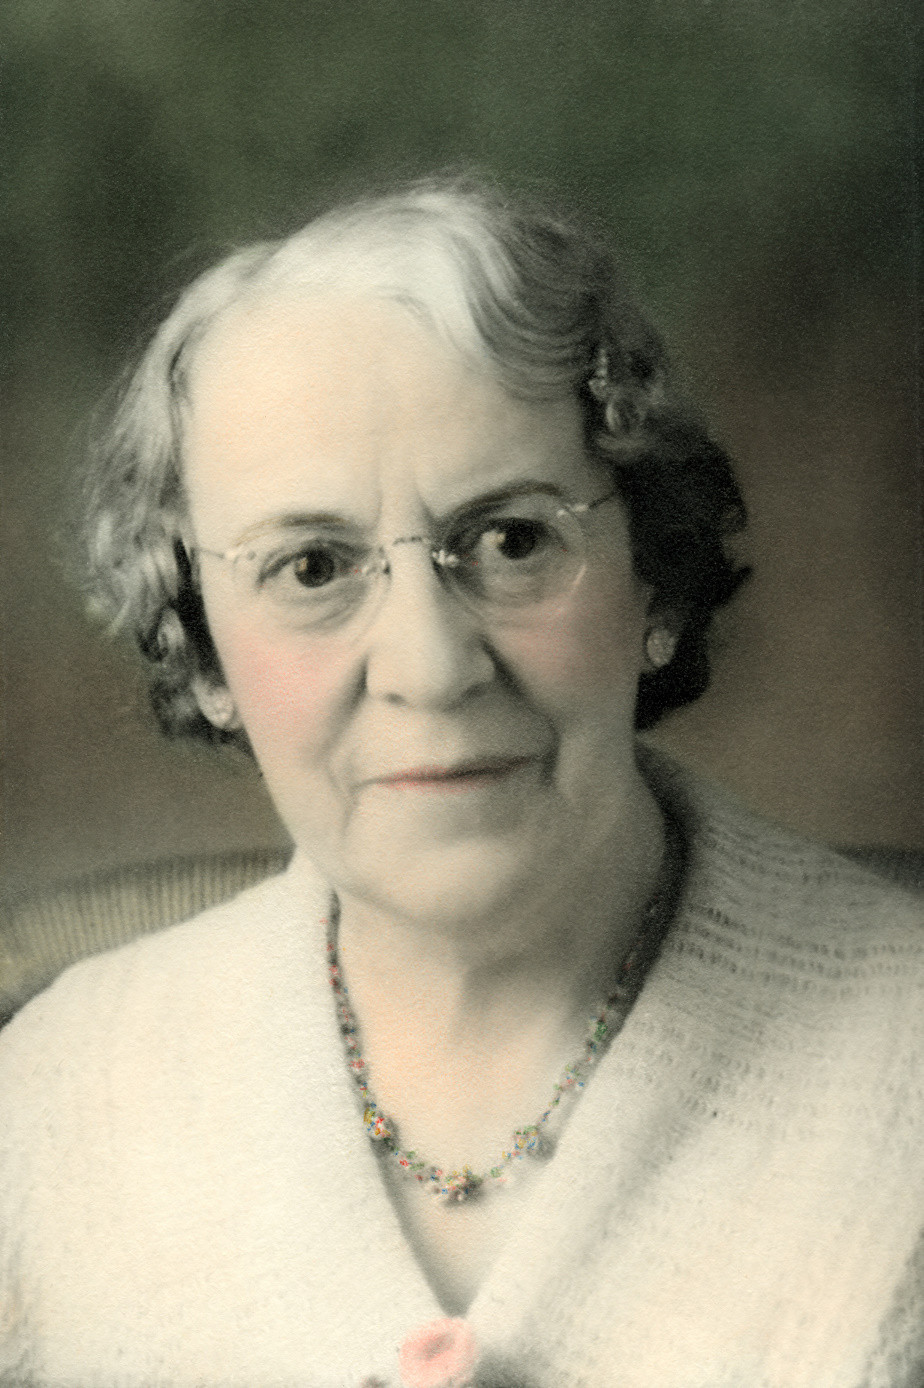
\includegraphics{minnie-e-raver.jpg}}
%Minnie E. Raver 1881-1977
%{[}/caption{]}

%\captionsetup[floatingfigure]{labelformat=empty}
%\begin{floatingfigure}[l]{0.29\textwidth}
%\centering
%\href{http://conceptcontrol.smugmug.com/People/Minnie-Raver/i-k6pnSJ4/A}{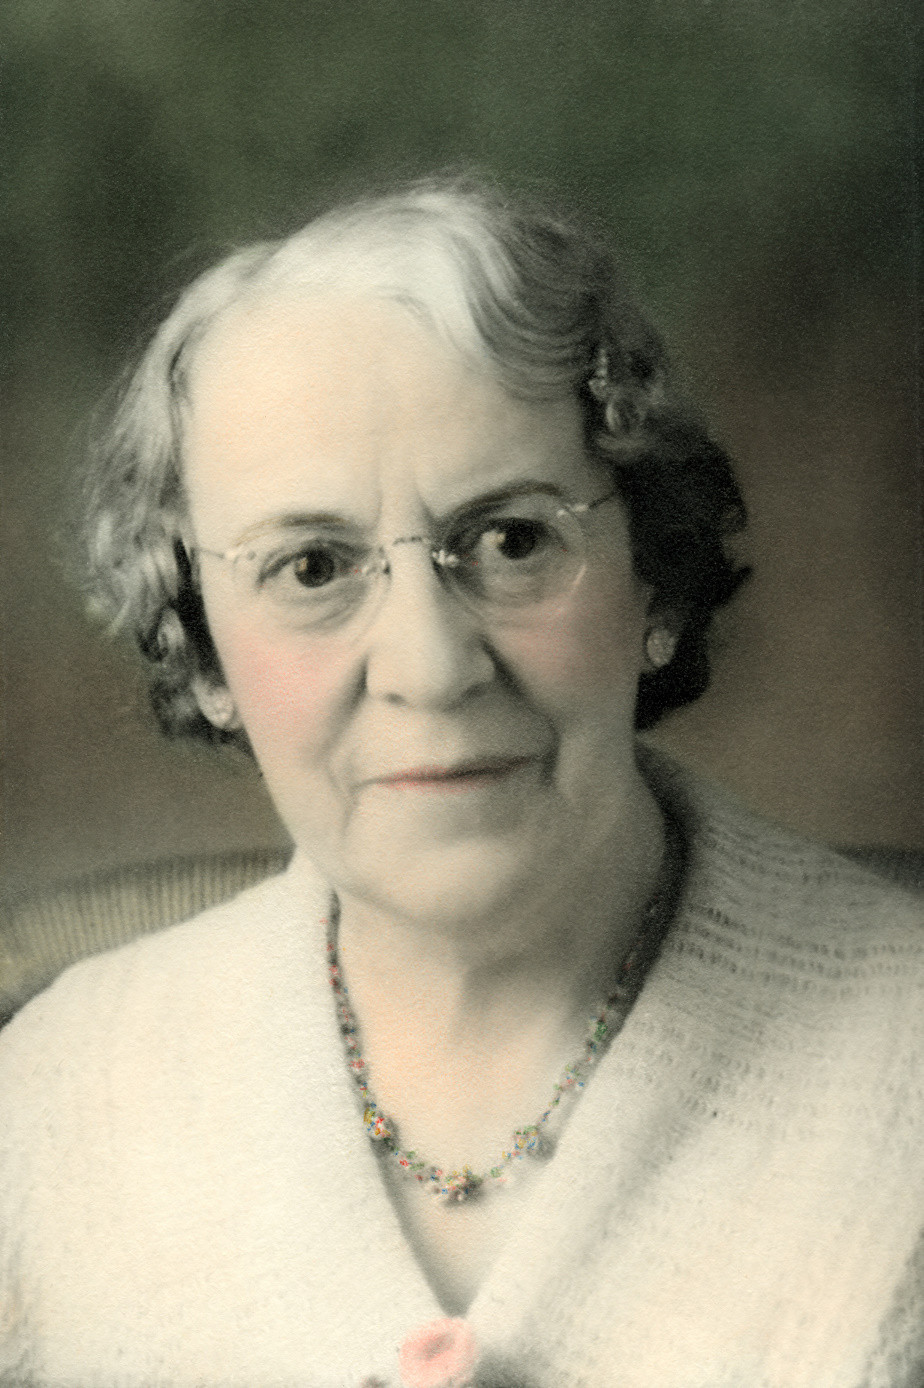
\includegraphics[width=0.26\textwidth]{minnie-e-raver.jpg}}
%\caption{Minnie Raver 1881-1977}
%\label{fig:4230X0}
%\end{floatingfigure} 

\captionsetup[figure]{labelformat=empty}
\begin{SCfigure}[1.5][!h]
\centering
\href{http://conceptcontrol.smugmug.com/People/Minnie-Raver/i-k6pnSJ4/A}{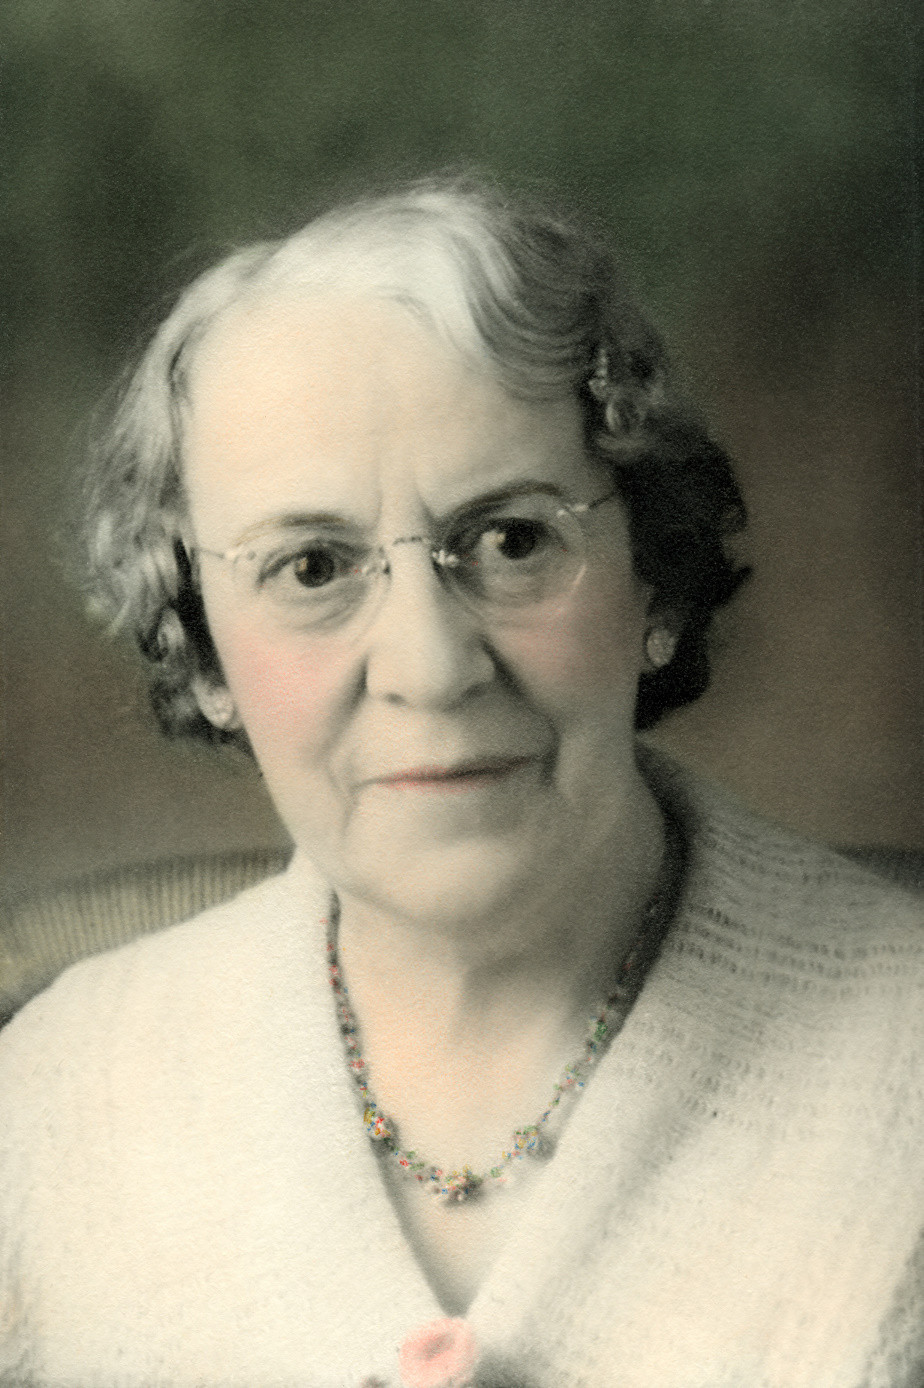
\includegraphics[width=0.26\textwidth]{minnie-e-raver.jpg}}
\caption{Minnie Raver 1881-1977. Minnie was one of my great-grandmothers. I only knew her as an old
lady.}
\label{fig:4230X0}
\end{SCfigure}


While going through my late mother's pictures I came across a box of my
great-grandmother Minnie's old photographs. When my great-grandmother
died in 1977 my grandmother
\href{http://conceptcontrol.smugmug.com/People/Grandparents-1/i-PBjmr7p/A}{Hazel}
took her pictures and stuffed them in her
\href{http://www.aetv.com/hoarders/}{Hoarder's level} junk filled
basement.\footnote{
If Hazel was alive today she would be a star on TV's Hoarders.
} After Hazel's death
\href{http://conceptcontrol.smugmug.com/People/The-Way-We-Were/i-Z64DmrR/A}{my
mother} recovered Minnie's pictures from Hazel's hoard and promptly
filed them with her pictures where they remained until I found them.
Minnie's pictures have already seen off three generations of my
ancestors and I'm next in line. Are they worth it?

Many of Minnie's pictures are over a hundred years old. The oldest
probably date to the 1870's or 1880's. Despite their age they're in
excellent condition. Obviously Minnie took care of her pictures and
thankfully Montana basements and attics are often high and dry. I spent
an entire day studying Minnie's pictures. Her old portraits are superb
examples of small studio 19\textsuperscript{th} and early
20\textsuperscript{th} century photography, see the following
\href{https://familysearch.org/pal:/MM9.1.1/F3SR-Q8S}{wedding portrait},
and her snapshots are candid shots of the people she knew and loved. All
of which brings me to my current problem. \emph{I don't know who these
people are!}


%{[}caption id=``attachment\_4298'' align=``aligncenter''  width=``454''{]}
%\href{http://conceptcontrol.smugmug.com/People/Minnie-Raver/i-Z7tfbBJ/A}{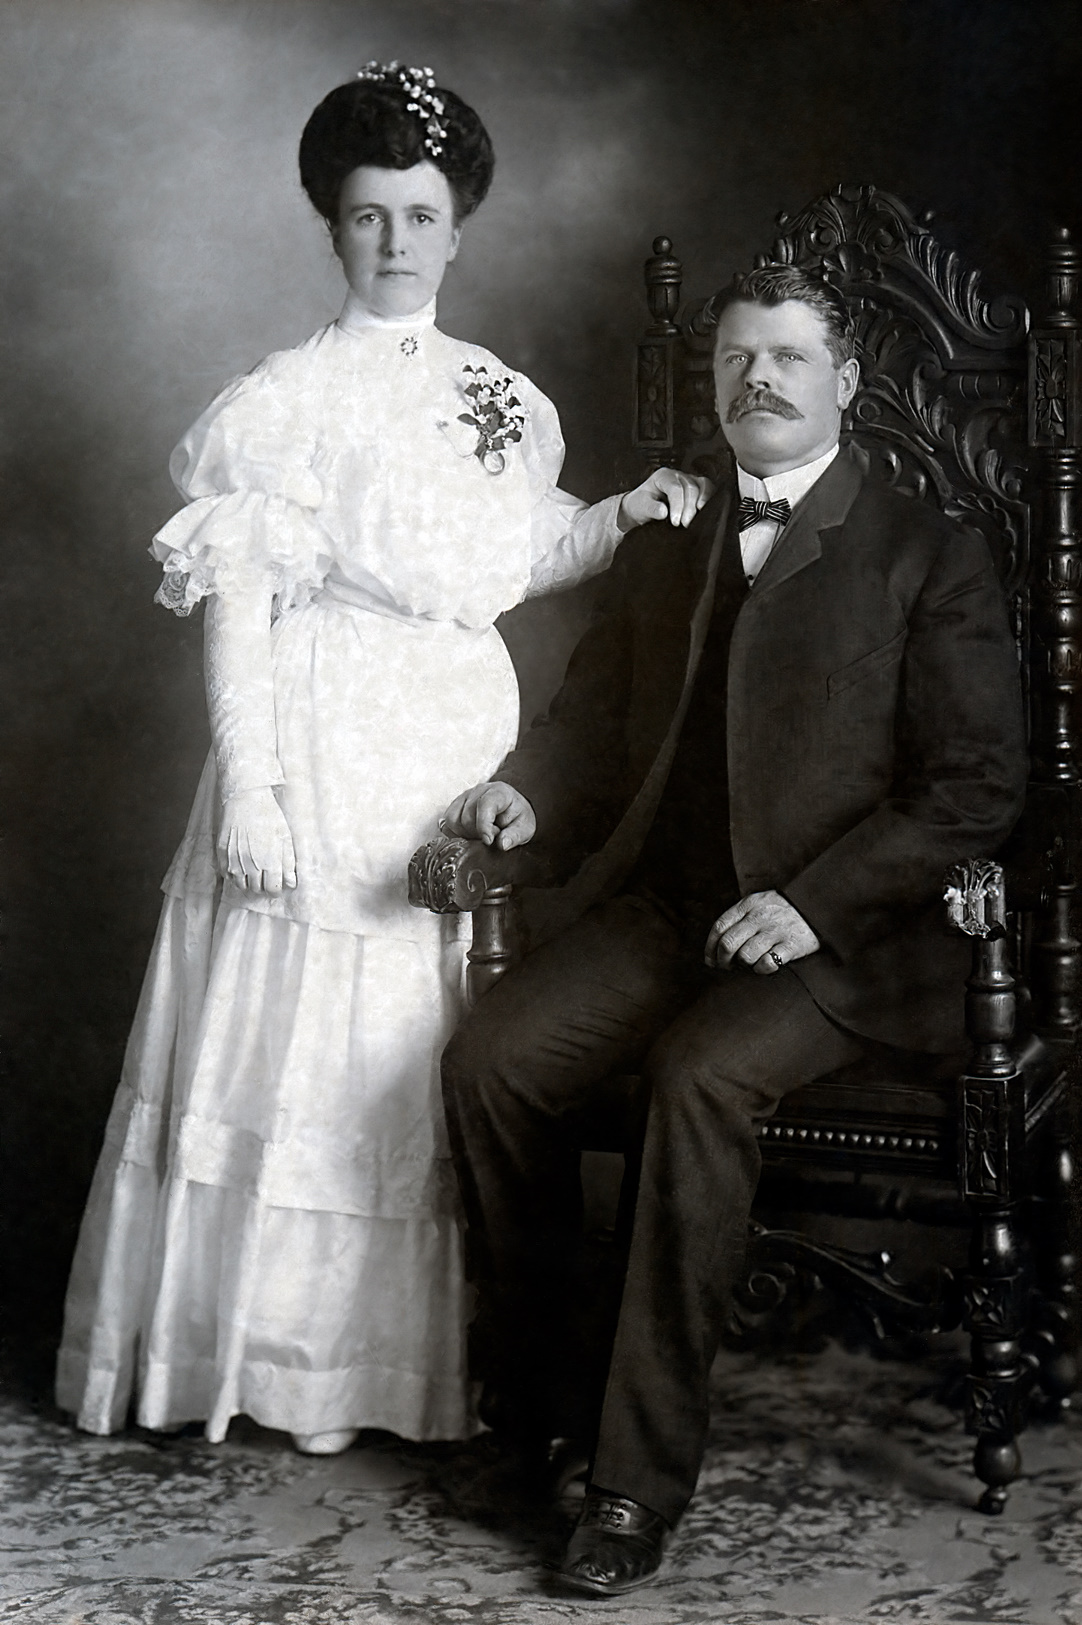
\includegraphics{callie-davis-frank-smelser-wedding-1905.jpg}}
%Callie Davis (Minnie's sister) and Frank Smelser wedding portrait
%1905.
%{[}/caption{]}

\captionsetup[figure]{labelformat=empty}
\begin{SCfigure}
%\begin{figure}[htbp]
%\begin{floatingfigure}[l]{0.38\textwidth}
\centering
\href{http://conceptcontrol.smugmug.com/People/Minnie-Raver/i-Z7tfbBJ/A}{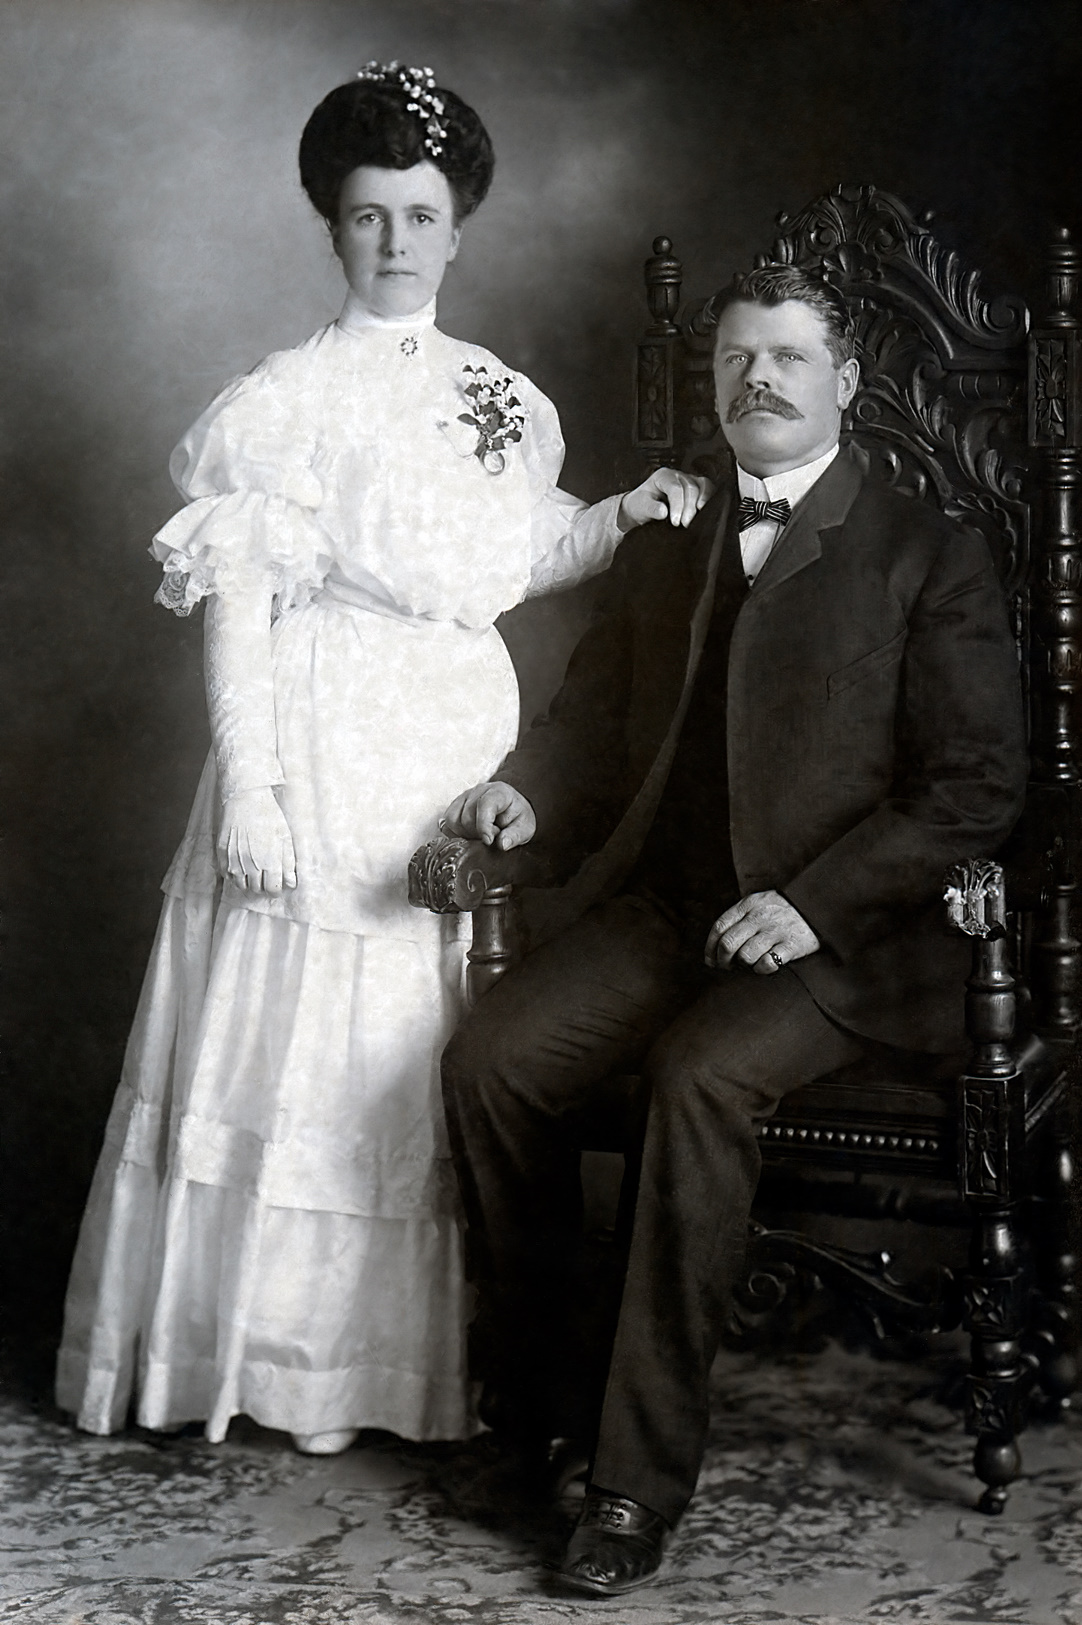
\includegraphics[width=0.35\textwidth]{callie-davis-frank-smelser-wedding-1905.jpg}}
\caption{Callie Davis (Minnie's sister) and Frank Smelser wedding portrait 1905}
\label{fig:4230X1}
%\end{figure}
%\end{floatingfigure}
\end{SCfigure}

I have never had much of an interest in family trees or the entire
quasi-delusional undertaking of genealogical research for the simple
reason that most of it is bullshit. \emph{The basic genealogical problem
is simple: people have always screwed around and then lied about it.}
When you get right down to it you cannot be certain, without DNA
testing, that your own parents are your biological parents. There are
good reasons to suspect that at least
\href{http://www.washingtoncitypaper.com/articles/8308/to-have-and-to-cuckold}{1\%
to 5\% of children} result from cuckolding~and for some social classes
it may be as~high as 30\%. In other words your daddy may not be who you
think it is! Cuckolding~varies with culture, time, socio-economic status
and so forth but it's rarely zero. A cuckolding rate of 5\% implies that
by the time you've traced your ancestors to the great-great-grandparent
level there is a 19\% chance that an alleged, perfectly documented,
ancestor is not really an ancestor. By the time we get back to the time
of Christ, roughly 100 generations, there's a 99.99\% chance that any
alleged ancestor is not really any ancestor. Genealogy without DNA is a
hollow dead-end.

As bad as cuckolding is it's~the least of our genealogical problems.
Genealogical records are incomplete, contain serious errors and are
often complete frauds. As late as the 19\textsuperscript{th} century the
settlement of estates was very sensitive to birth order. If you were a
first-born son you got everything while your baby brother got squat. It
was even worse for women; they got less than squat. In such an
environment there is a powerful incentive to forge records. Old
handwritten documents may look official to modern eyes but you cannot
assume they're accurate. With a well-placed bribe first-born Johnnie
suddenly disappears from the record. \emph{People have always lied about
the important things.}

Given all these obvious problems I usually ignore people going on about
the exploits of their glorious ancestors. Your roots are unreliable
people! You really don't know who your great-great-great granny was and
if you insist on telling tales about her I will insist on DNA evidence.
I know that many of the dead in Minnie's pictures are \emph{probably}
blood relatives and some are probably direct great-great or greater
grandparents. I cannot be 100\% sure they're genetic ancestors but I can
follow obvious document breadcrumbs and learn enough about these people
to attach stories to their pictures.

I wasn't looking forward to the giant chore of scanning, restoring and
researching Minnie's pictures\footnote{
Despite their good condition it was still a lot of work to restore the
images posted here. To judge what I had contend with browse this
gallery of  \href{http://conceptcontrol.smugmug.com/Themes/Manipulations/Restorations-1}{before
and after diptychs}.
}  but
following breadcrumbs was more interesting than expected. It turns out
that there's~a lot of dead people on the internet. When I started
looking for death and marriage records I immediately came across a
cemetery record for
\href{http://www.findagrave.com/cgi-bin/fg.cgi?page=gr\&GSln=baker\&GSfn=evelyn+\&GSmn=v\&GSbyrel=all\&GSdyrel=all\&GSst=28\&GScnty=1627\&GScntry=4\&GSob=n\&GRid=110246189\&df=all\&}{my
own recently deceased mother}. It was surprising~to find her so soon.
There's an active world-wide~ghoulish~group of people photographing
cemetery monuments and posting their findings online. It's ironic but a
\href{http://en.wikipedia.org/wiki/Find\_a\_Grave}{Facebook for the
dead} preceded the Facebook for the living. Starting with my mother I
backtracked through my alleged ancestors looking for a ``Lydia.''
~``Lydia''~was scrawled on the back of what looked like~the oldest of
Minnie's pictures.


%{[}caption id=``attachment\_4251'' align=``aligncenter''  width=``353''{]}
%\href{http://conceptcontrol.smugmug.com/People/Minnie-Raver/i-FWtqBg4/A}{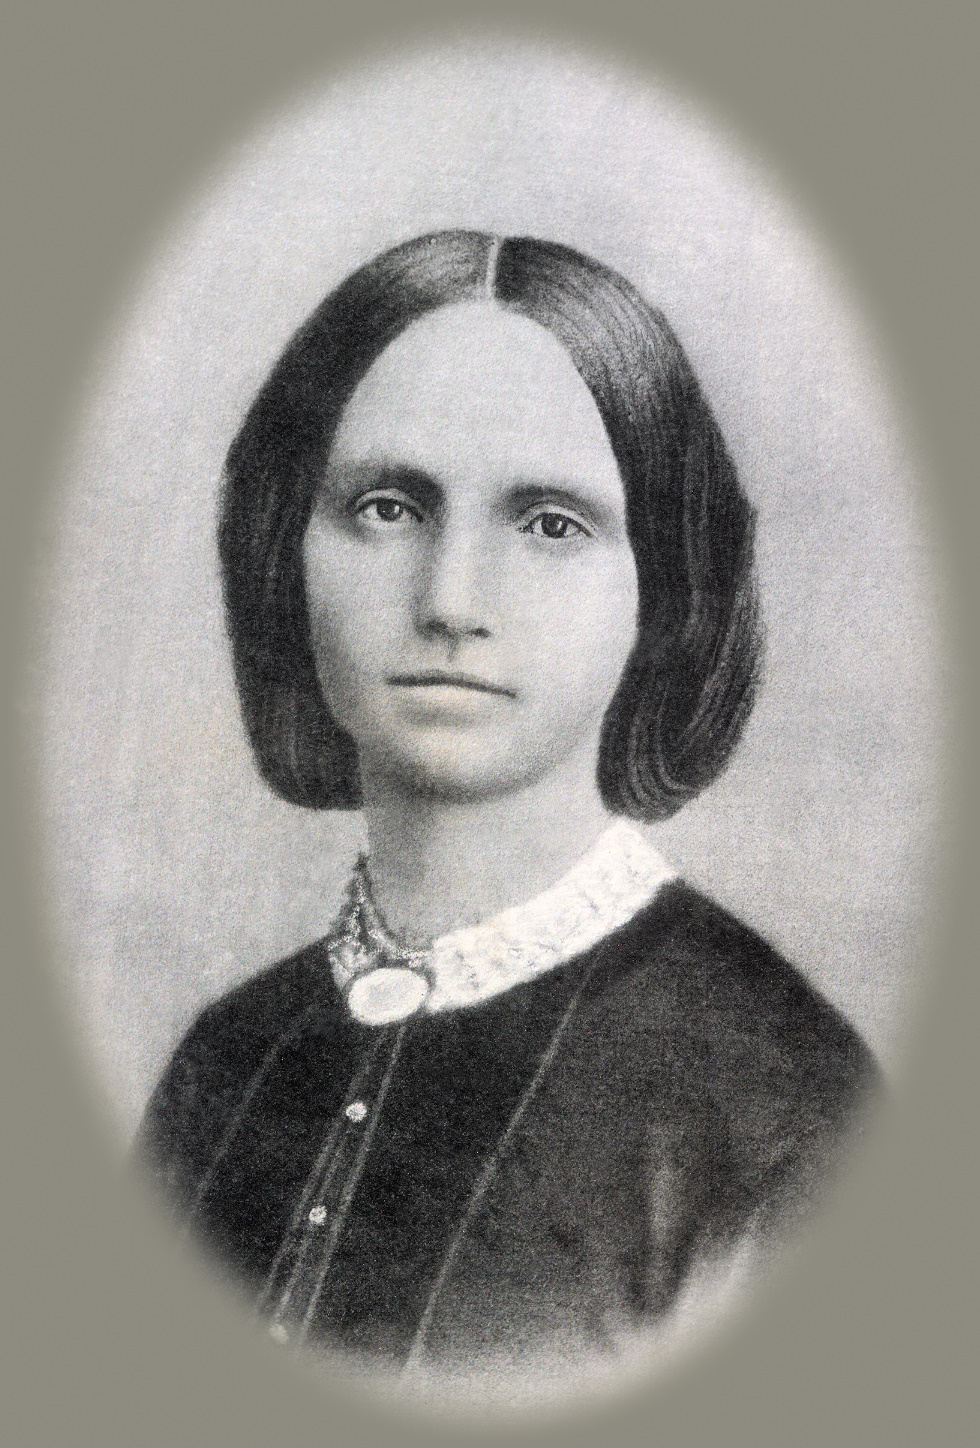
\includegraphics{lydia-ayres.jpg}}
%Lydia Jane Ayres 1839-unknown
%{[}/caption{]}

\begin{SCfigure}
%\begin{figure}[htbp]
%\begin{floatingfigure}[r]{0.38\textwidth}
\centering
\href{http://conceptcontrol.smugmug.com/People/Minnie-Raver/i-FWtqBg4/A}{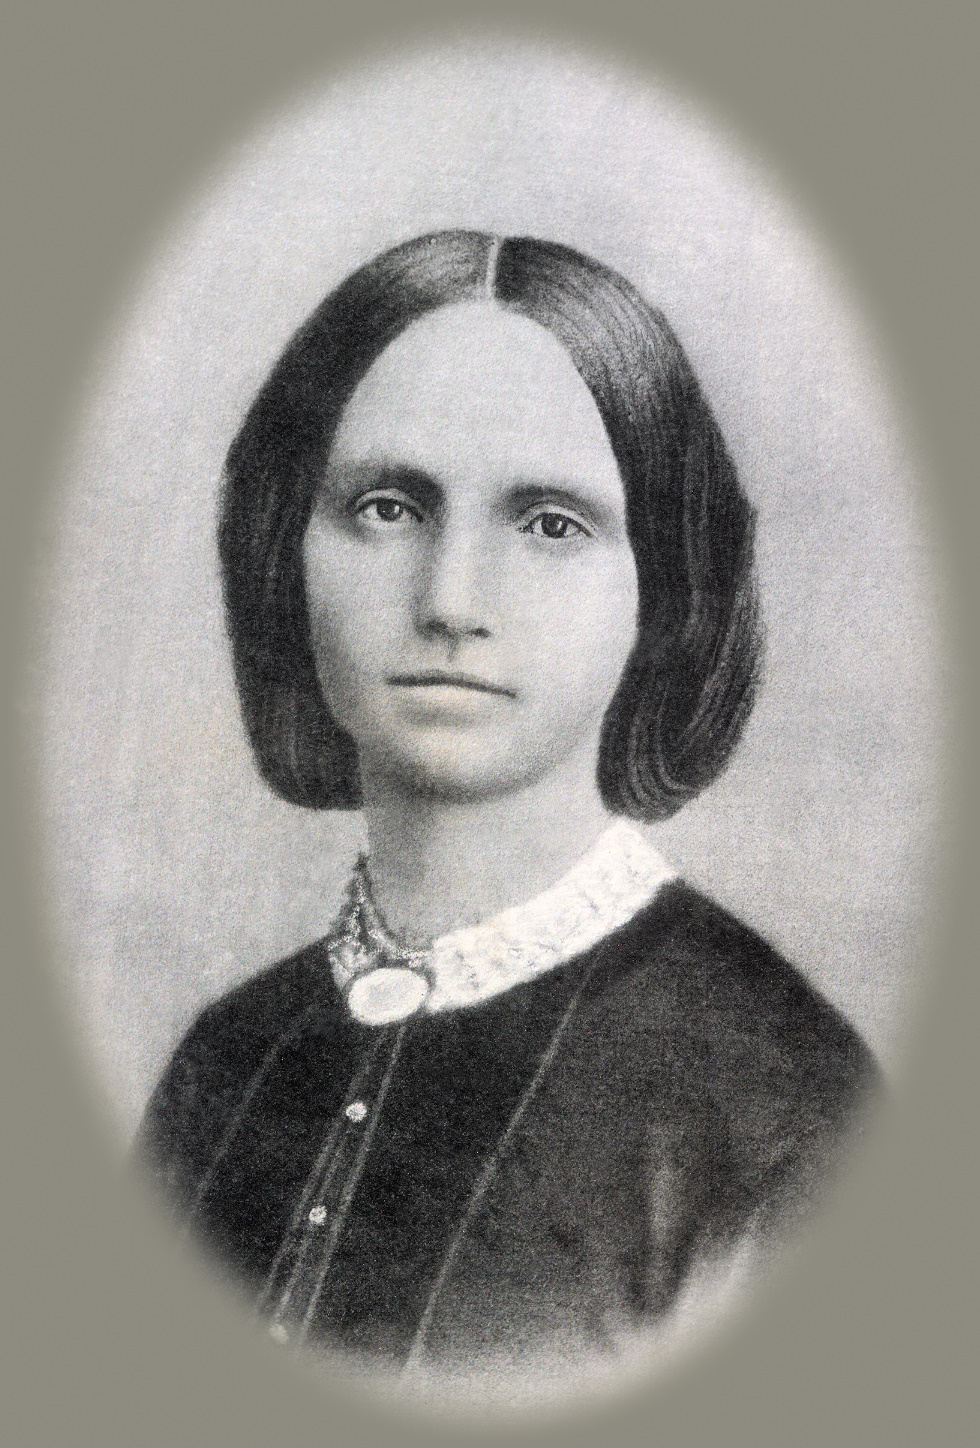
\includegraphics[width=0.35\textwidth]{lydia-ayres.jpg}}
\caption{Lydia Jane Ayres 1839-unknown}
\label{fig:4230X2}
%\end{figure}
%\end{floatingfigure}
\end{SCfigure}

If the records are correct I believe this ``Lydia'' is Lydia Jane Ayres.
There is a very good chance that Lydia is one of my great-great
grandmothers.
\href{https://familysearch.org/pal:/MM9.1.1/XLPB-DF8}{Lydia married
Albert F. Raver} in 1863 in Brant Ontario. Albert was the mother of
Minnie's husband
\href{https://familysearch.org/pal:/MM9.1.1/F3Q3-45X}{Bert Raver}.

I didn't find any pictures of Albert Raver in Minnie's collection and
that's too bad because I~suspect Albert had an eye for the babes. I
looked for his death record and found this
\href{https://familysearch.org/pal:/MM9.1.1/MVLY-WLB}{confusing census
entry}. Here was an Albert F. Raver with exactly the same age and birth
origin remarried to a Lydia L. Raver. At first I thought it was a
mistake but Albert's marriage to Lydia L. Ayres was in 1906. That did
not compute. Then I remembered a story my grandmother Hazel told me
years ago when we were talking about her grandparents. She told me that
one of her grandfathers married twice to two women with the same first
and last names. She complained about how difficult this made sorting
Christmas and birthday cards. I cannot remember if the name was Lydia
Ayres but what are the chances? It seems Albert married~ Lydia Jane
Ayres in 1863. Somehow~they parted ways and later, at the age of 68,
Albert remarried in 1906 a younger Lydia L. Ayres. Having been divorced
and remarried myself I can only marvel at Albert's ingenuity. The last
thing you want to do in your senile dotage is call a second wife by your
first wife's name. Before social security that could have been a fatal
mistake.
\href{http://www.findagrave.com/cgi-bin/fg.cgi?page=gr\&GRid=89404051}{Randy
old Albert} neatly dodged that bullet.

The randiness was not confined to the Raver branch. Equally intriguing
is this old portrait of ``dad's old sweetheart.'' Here Minnie is likely
referring to her own father and my great-great granddaddy
\href{http://www.findagrave.com/cgi-bin/fg.cgi?page=gr\&GSln=Davis\&GSfn=Howell\&GSmn=C\&GSby=1850\&GSbyrel=after\&GSdy=1950\&GSdyrel=before\&GSst=28\&GScntry=4\&GSob=n\&GRid=67837689\&df=all\&}{Howell
Cobb Davis}. Screwing around, contrary to boomer mythology, wasn't
invented in the 1960's.


%{[}caption id=``attachment\_4292'' align=``aligncenter''  width=``486''{]}
%\href{http://conceptcontrol.smugmug.com/People/Minnie-Raver/i-GGmLK2W/A}{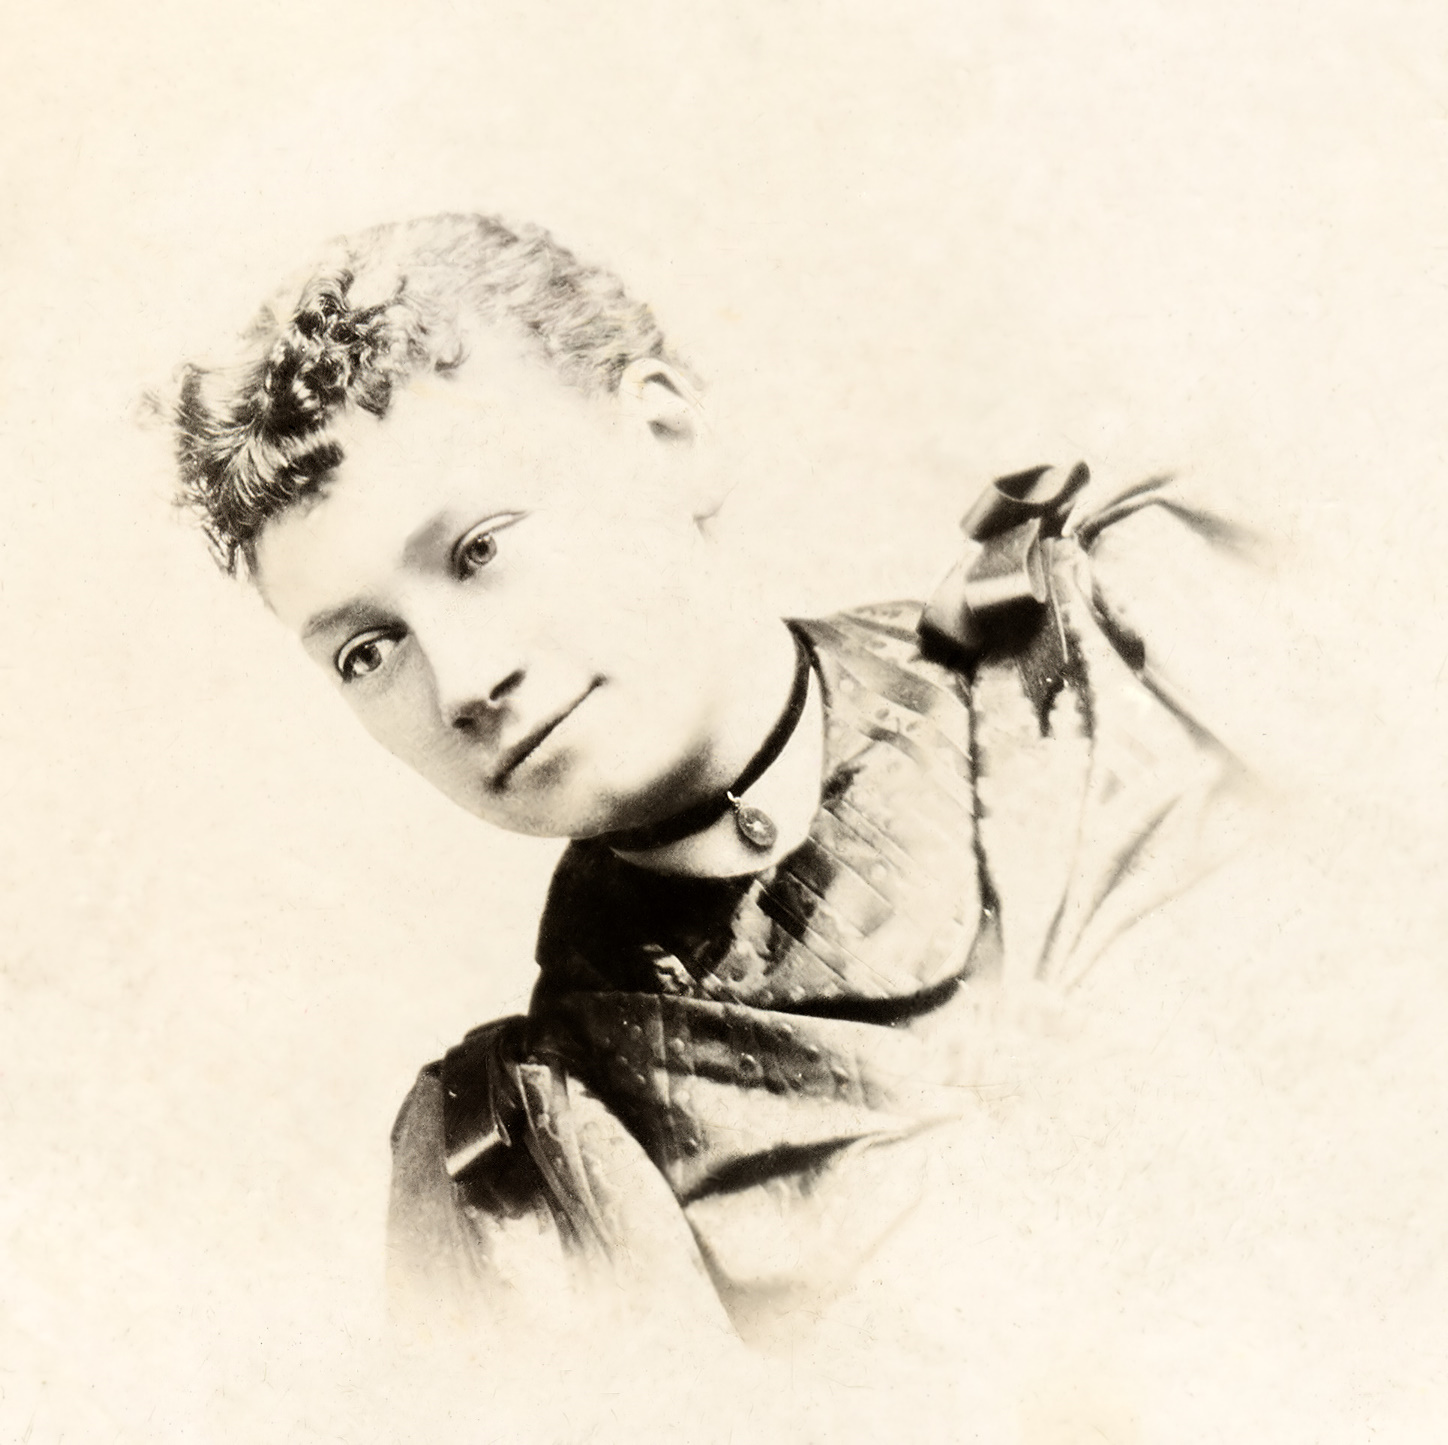
\includegraphics{dad-old-sweetheart.jpg}}
%``Dad's old sweetheart.'' Probably an old girl friend of Howell Cobb
%Davis.
%{[}/caption{]}

\begin{SCfigure}
%\begin{figure}[htbp]
\centering
\href{http://conceptcontrol.smugmug.com/People/Minnie-Raver/i-GGmLK2W/A}{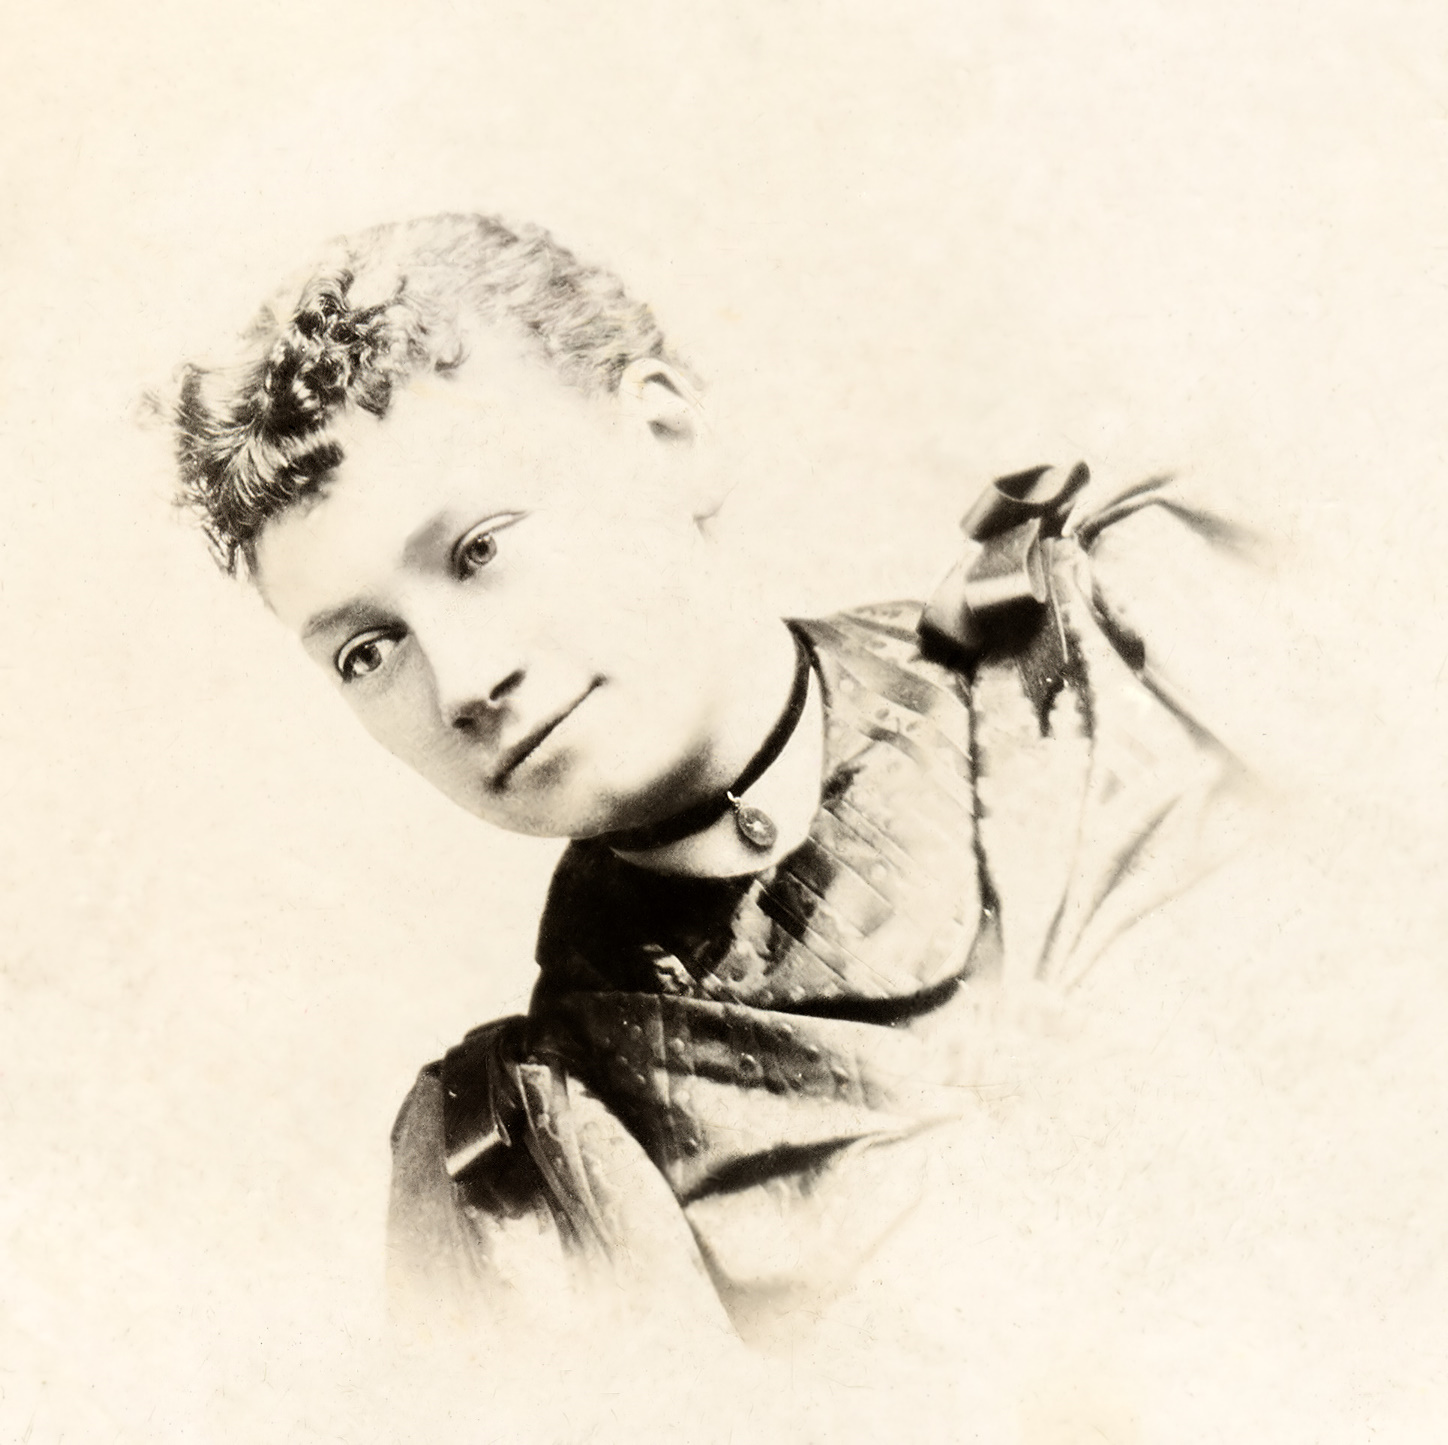
\includegraphics[width=0.35\textwidth]{dad-old-sweetheart.jpg}}
\caption{``Dad's old sweetheart.'' Probably an old girl friend of Howell Cobb Davis.}
\label{fig:4230X3}
%\end{figure}
\end{SCfigure}


Minnie lived to 96. I was in my twenties when she died so I remember
some of the people in her snapshots. Here's Minnie with her
\href{http://www.findagrave.com/cgi-bin/fg.cgi?page=gr\&GRid=61581142}{first-born
son Vernon} standing in Marble Canyon Arizona in 1949. I knew~Vernon as
a boy. He always posed exactly like you see him her.


%{[}caption id=``attachment\_4261'' align=``aligncenter''  width=``1154''{]}
%\href{http://conceptcontrol.smugmug.com/People/Minnie-Raver/i-DTmc5Zb/A}{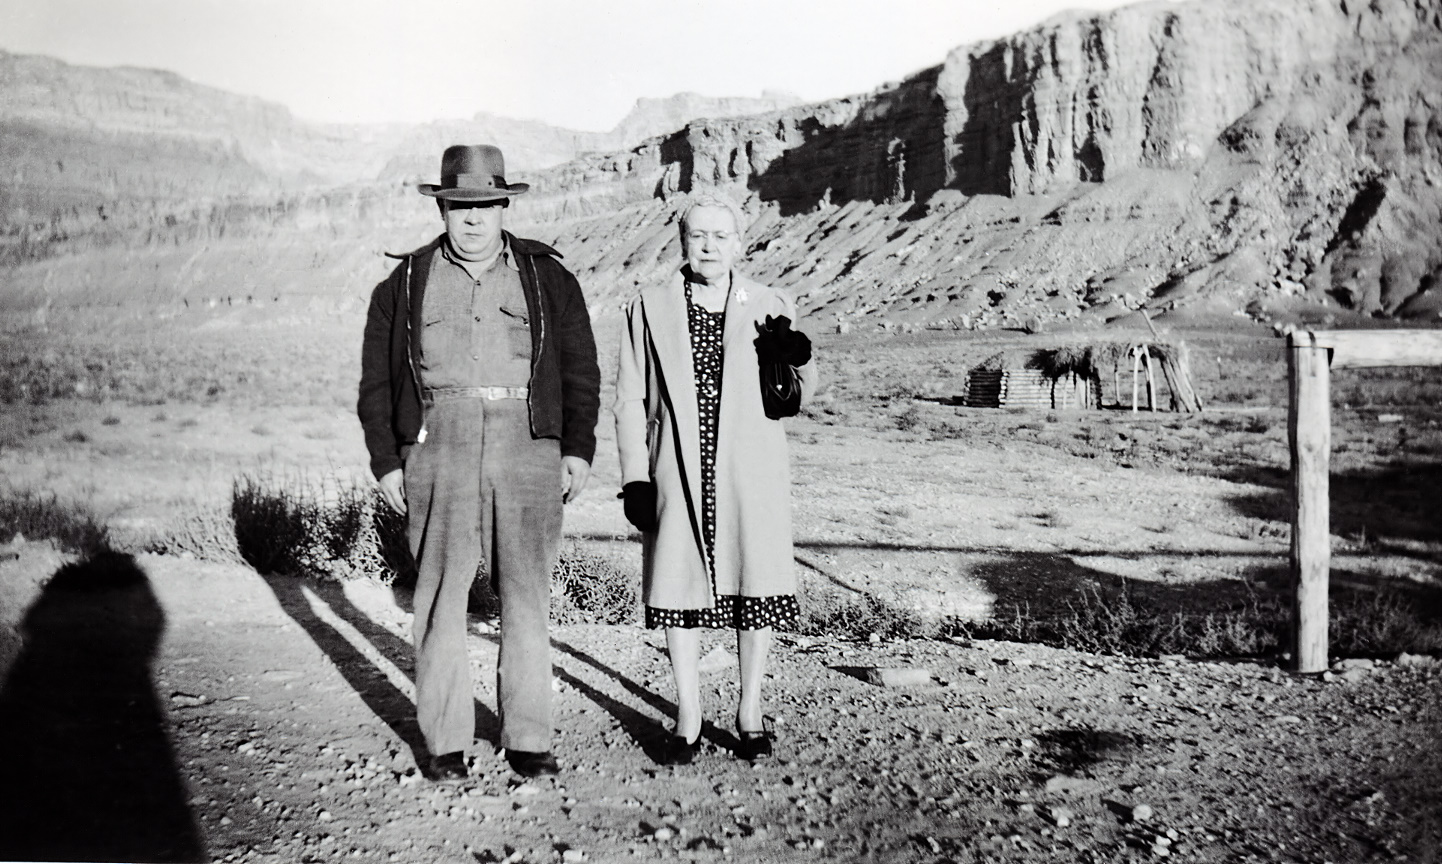
\includegraphics{vernon-minnie-raver-marble-canyon-arizona-1949.jpg}}
%Vernon and Minnie Raver Marble Canyon Arizona 1949
%{[}/caption{]}

\begin{SCfigure}
%\begin{figure}[htbp]
\centering
\href{http://conceptcontrol.smugmug.com/People/Minnie-Raver/i-DTmc5Zb/A}{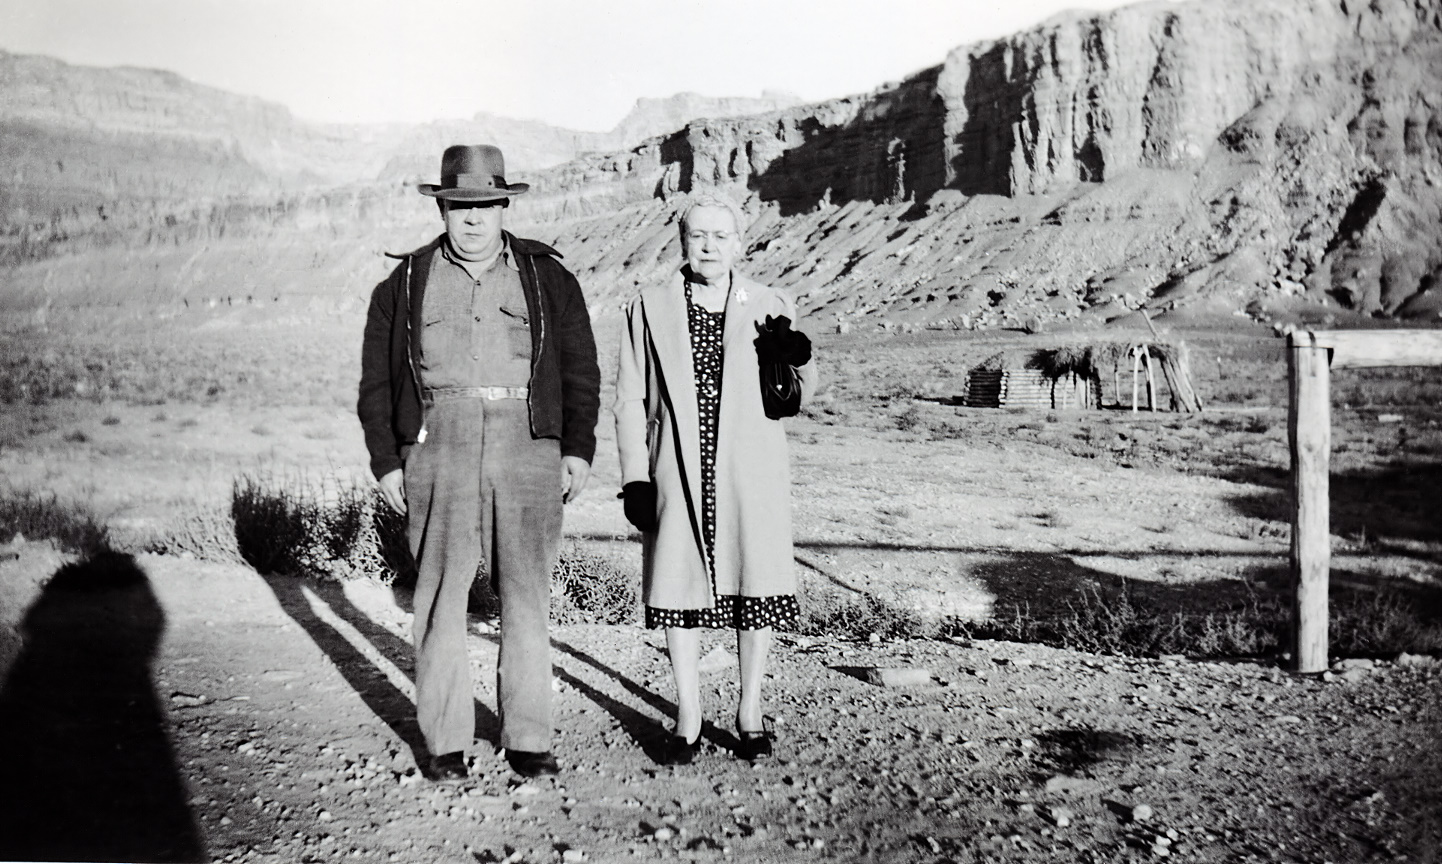
\includegraphics[width=0.50\textwidth]{vernon-minnie-raver-marble-canyon-arizona-1949.jpg}}
\caption{Vernon and Minnie Raver Marble Canyon Arizona 1949}
\label{fig:4230X4}
%\end{figure}
\end{SCfigure}


You can read the poor guys mind. ``Do you really need another picture?
Well if that's how it's going be I'm going to assume my petulant spoiled
fat boy pose.'' You cannot blame Vernon. His photographic life got off
to a dreadful start. Look at this gem.


%{[}caption id=``attachment\_4286'' align=``aligncenter''  width=``412''{]}
%\href{http://conceptcontrol.smugmug.com/People/Minnie-Raver/i-pms8BTb/A}{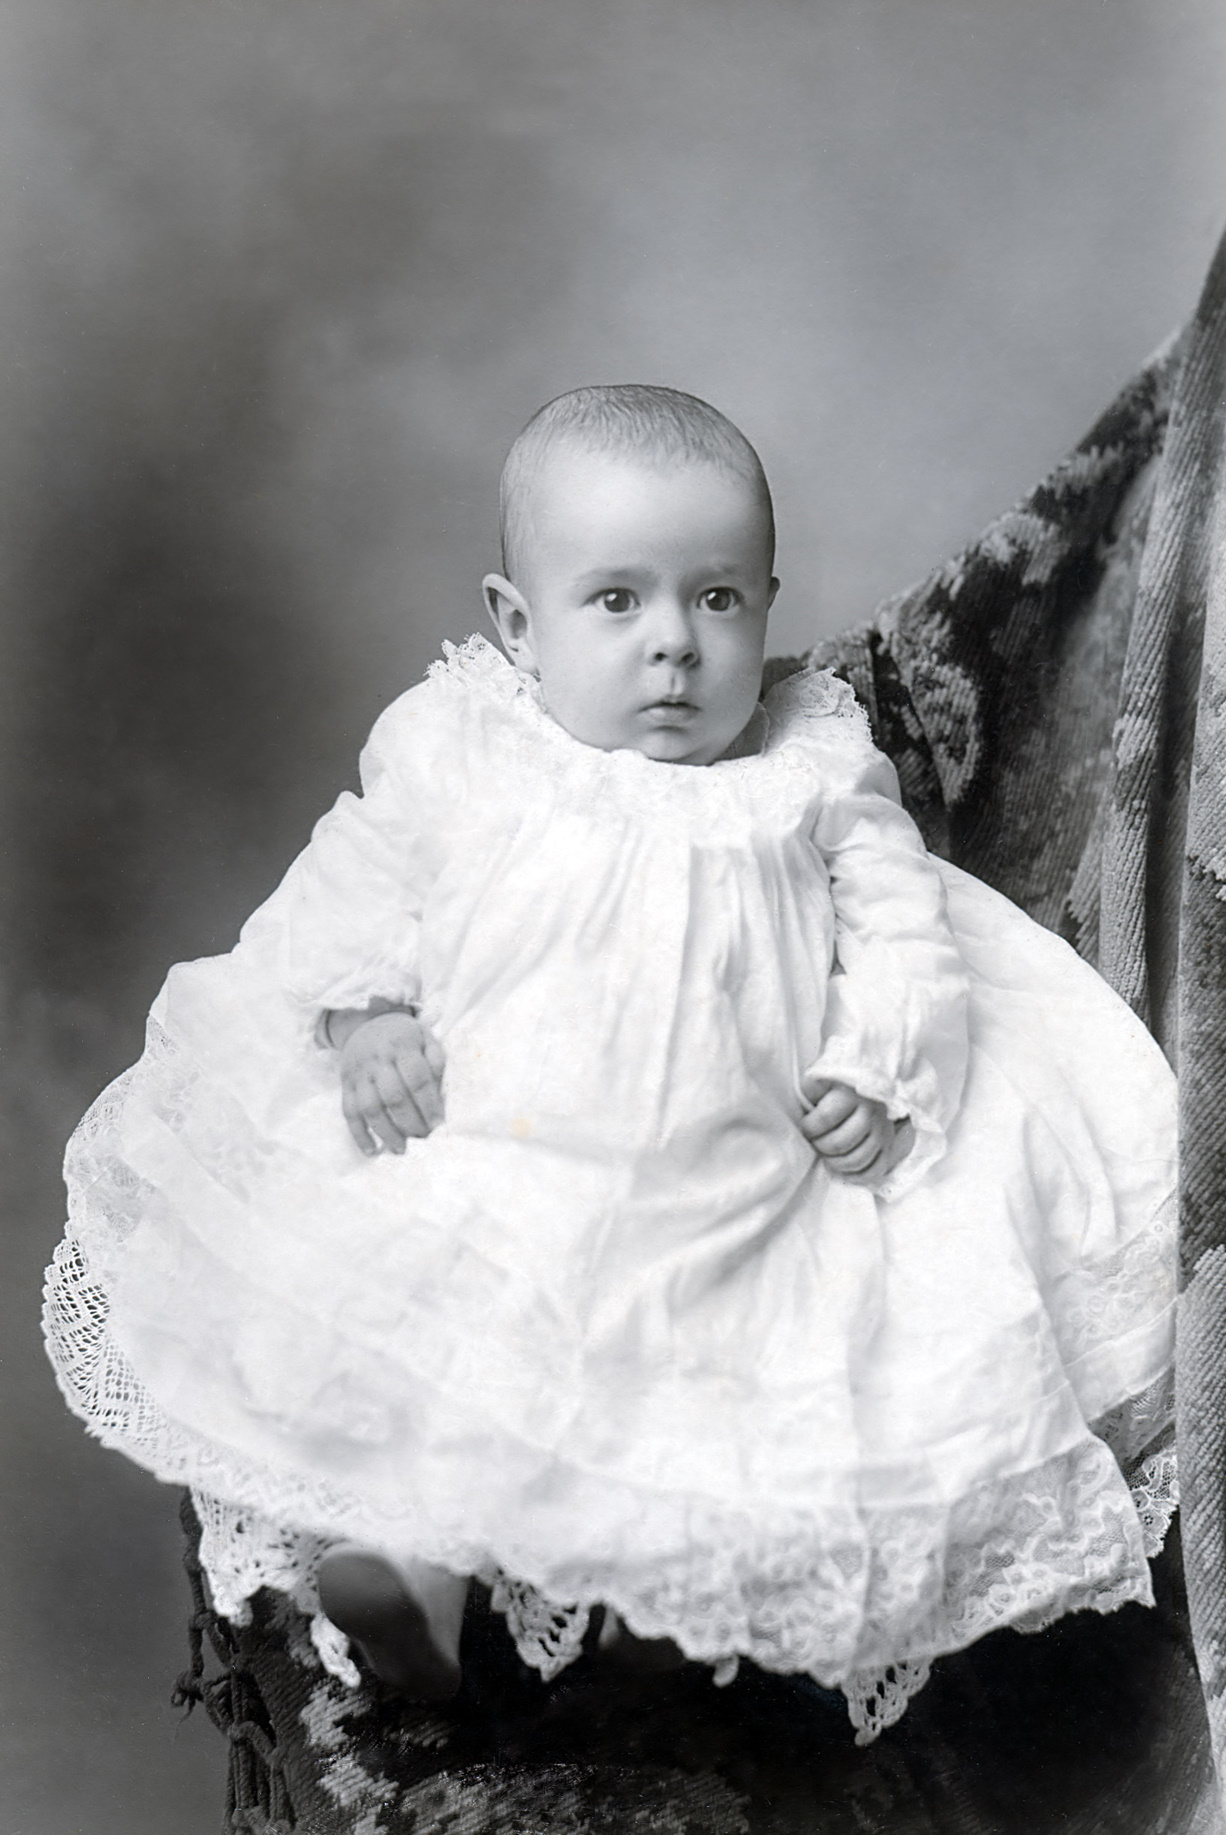
\includegraphics{vernon-raver-hazels-brother.jpg}}
%Vernon F. Raver 1904-1964
%{[}/caption{]}

\begin{SCfigure}
%\begin{figure}[htbp]
\centering
\href{http://conceptcontrol.smugmug.com/People/Minnie-Raver/i-pms8BTb/A}{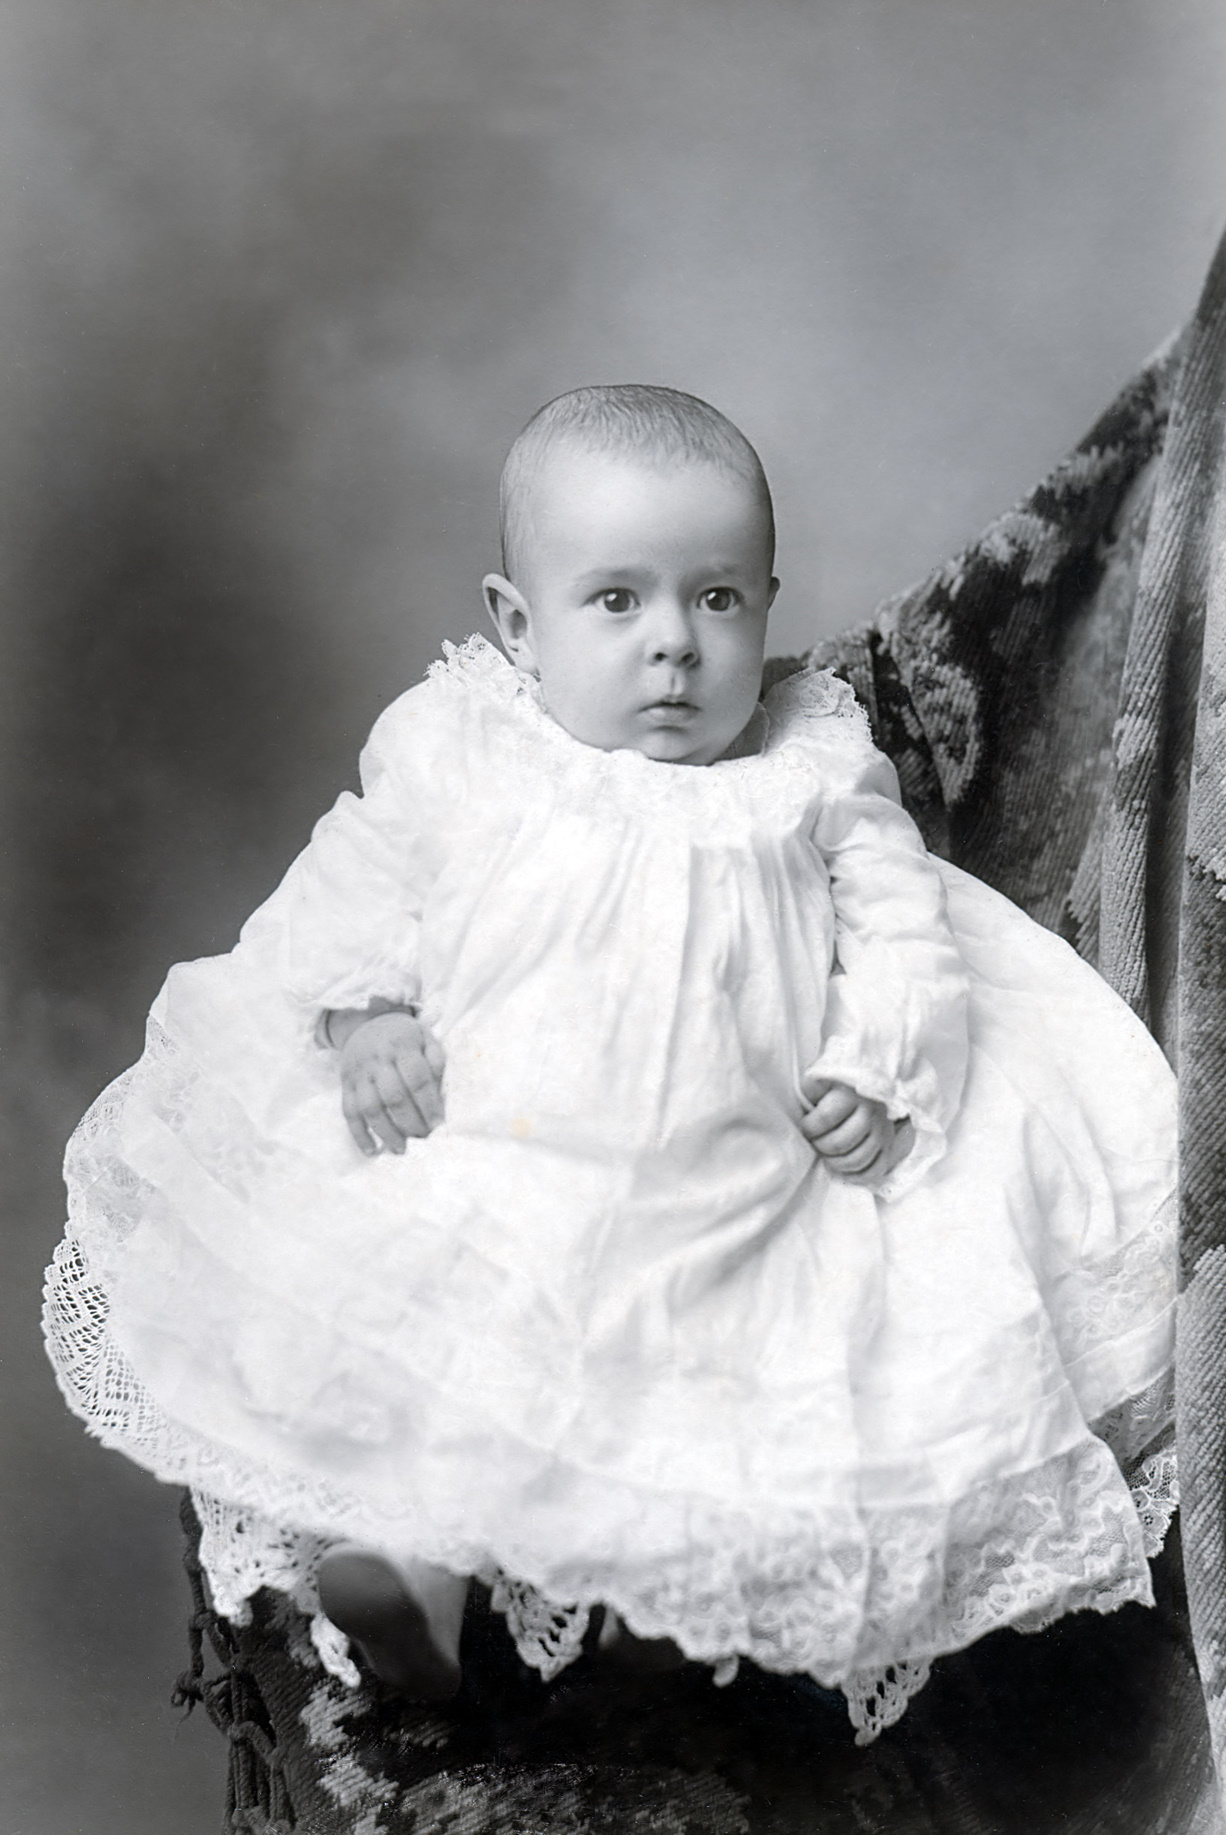
\includegraphics[width=0.35\textwidth]{vernon-raver-hazels-brother.jpg}}
\caption{Vernon F. Raver 1904-1964}
\label{fig:4230X5}
%\end{figure}
\end{SCfigure}


In the early 20\textsuperscript{th} century women liked to dress up
their baby boys as girls. Vernon got the full girly treatment. You
cannot blame him for being scarred for life after such trauma. Here's a
clue ladies. Boys are not girls. Gender is not arbitrary. People that
assert the contrary are idiots.~Sorry if that sounds like
\href{http://www.policymic.com/articles/44479/mansplaining-101-how-to-discuss-politics-and-feminism-without-acting-like-a-jackass}{mansplaining};~the
truth is not always polite.

I doubt I'll ever get through Minnie's pictures. There are hundreds of
images to scan, restore and research. I just don't have the time or
energy but in the years ahead I will occasionally pick out and upload
attractive images. Here's
\href{http://conceptcontrol.smugmug.com/People/Minnie-Raver}{the gallery
to follow} if you're interested.

%\begin{center}\rule{3in}{0.4pt}\end{center}
%
%\begin{enumerate}
%\item
%  If Hazel was alive today she would be a star on TV's
%  Hoarders.\hyperref[fnref1]{↩}
%\item
%  Despite their good condition it was still a lot of work to restore the
%  images posted here. To judge what I had contend with browse this
%  gallery of
%  \href{http://conceptcontrol.smugmug.com/Themes/Manipulations/Restorations-1}{before
%  and after diptychs}.\hyperref[fnref2]{↩}
%\end{enumerate}

%\captionsetup[floatingfigure]{labelformat=empty}
%\begin{figure}[htbp]
%\begin{floatingfigure}[l]{0.25\textwidth}
%\centering
%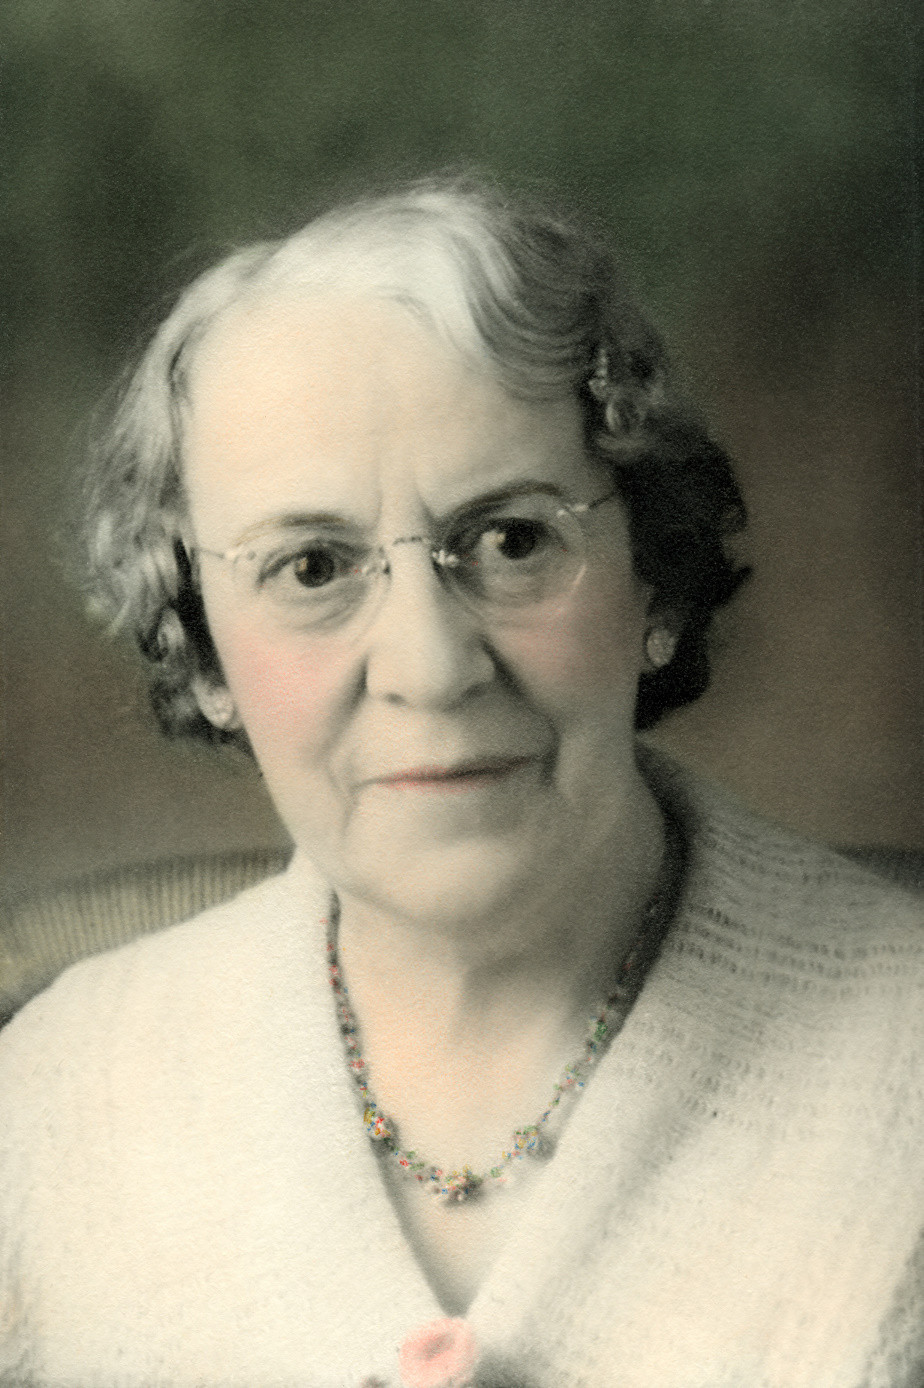
\includegraphics[width=0.23\textwidth]{minnie-e-raver.jpg}
%\caption{~~~IMCAPTION~~~}
%\label{fig:4230X0}
%\end{floatingfigure}
%\end{figure}

%\captionsetup[floatingfigure]{labelformat=empty}
%\begin{figure}[htbp]
%\begin{floatingfigure}[l]{0.25\textwidth}
%\centering
%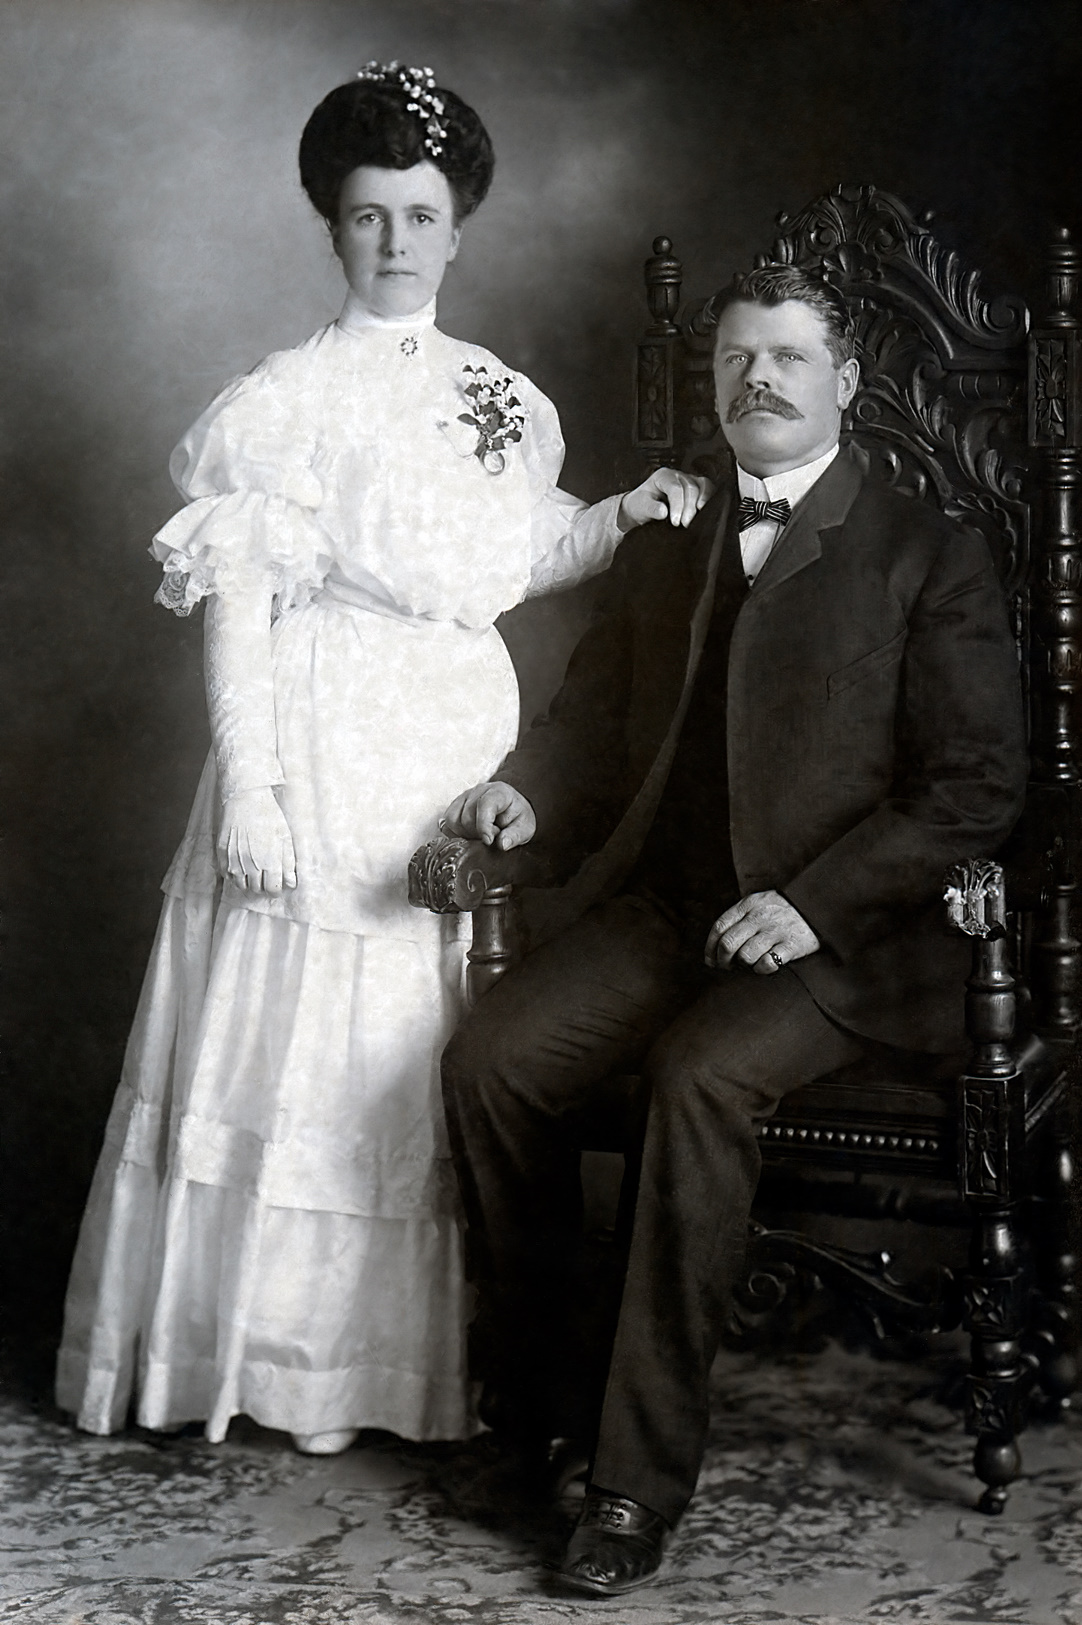
\includegraphics[width=0.23\textwidth]{callie-davis-frank-smelser-wedding-1905.jpg}
%\caption{~~~IMCAPTION~~~}
%\label{fig:4230X1}
%\end{floatingfigure}
%\end{figure}

%\captionsetup[floatingfigure]{labelformat=empty}
%\begin{figure}[htbp]
%\begin{floatingfigure}[l]{0.25\textwidth}
%\centering
%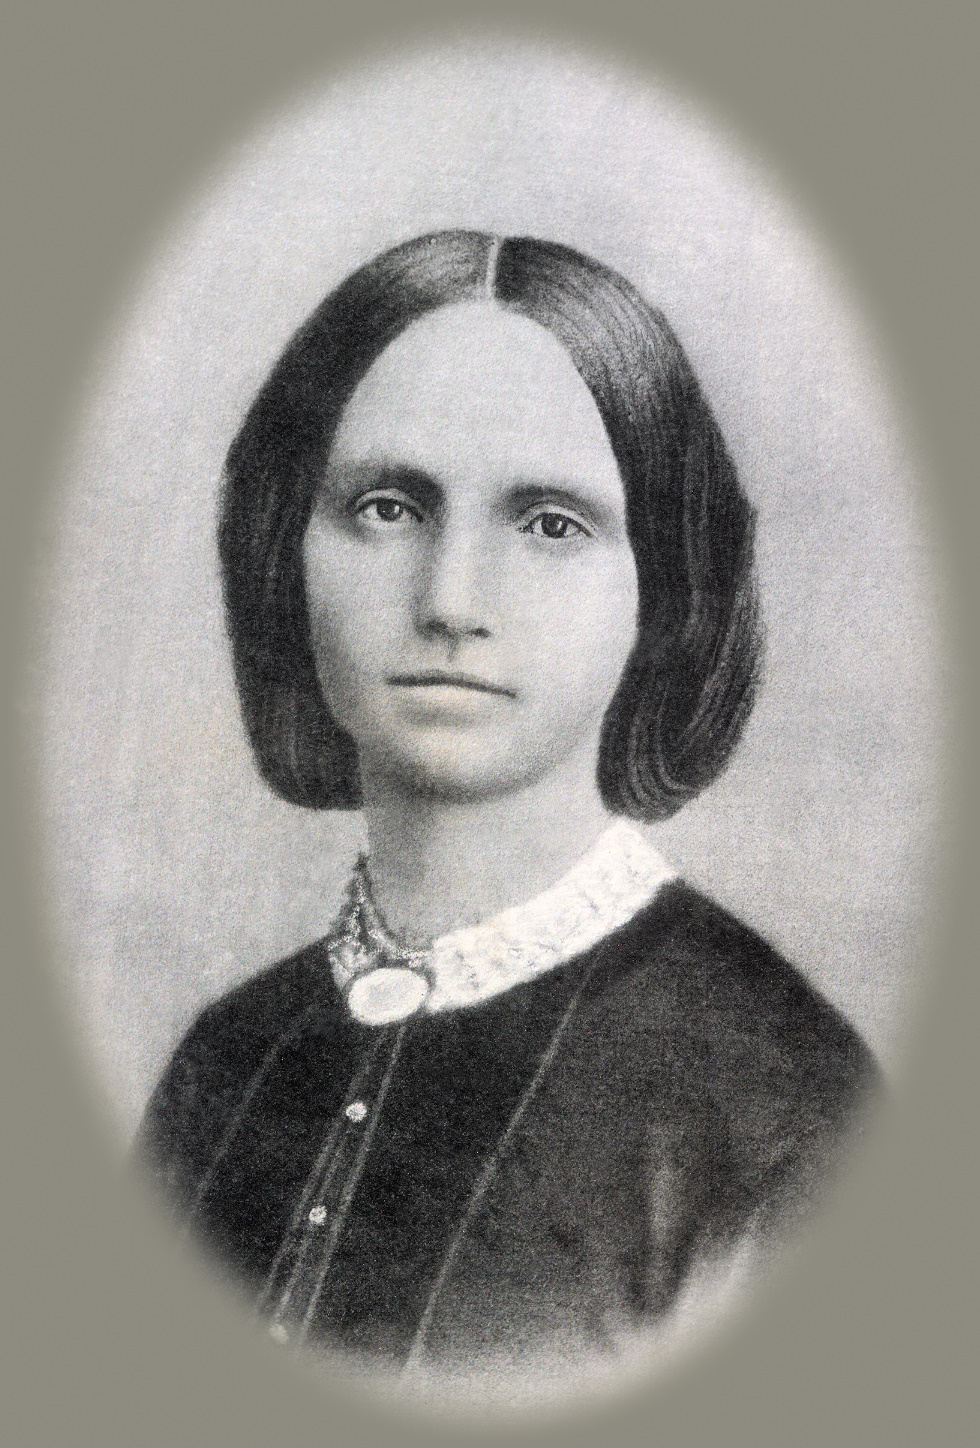
\includegraphics[width=0.23\textwidth]{lydia-ayres.jpg}
%\caption{~~~IMCAPTION~~~}
%\label{fig:4230X2}
%\end{floatingfigure}
%\end{figure}

%\captionsetup[floatingfigure]{labelformat=empty}
%\begin{figure}[htbp]
%\begin{floatingfigure}[l]{0.25\textwidth}
%\centering
%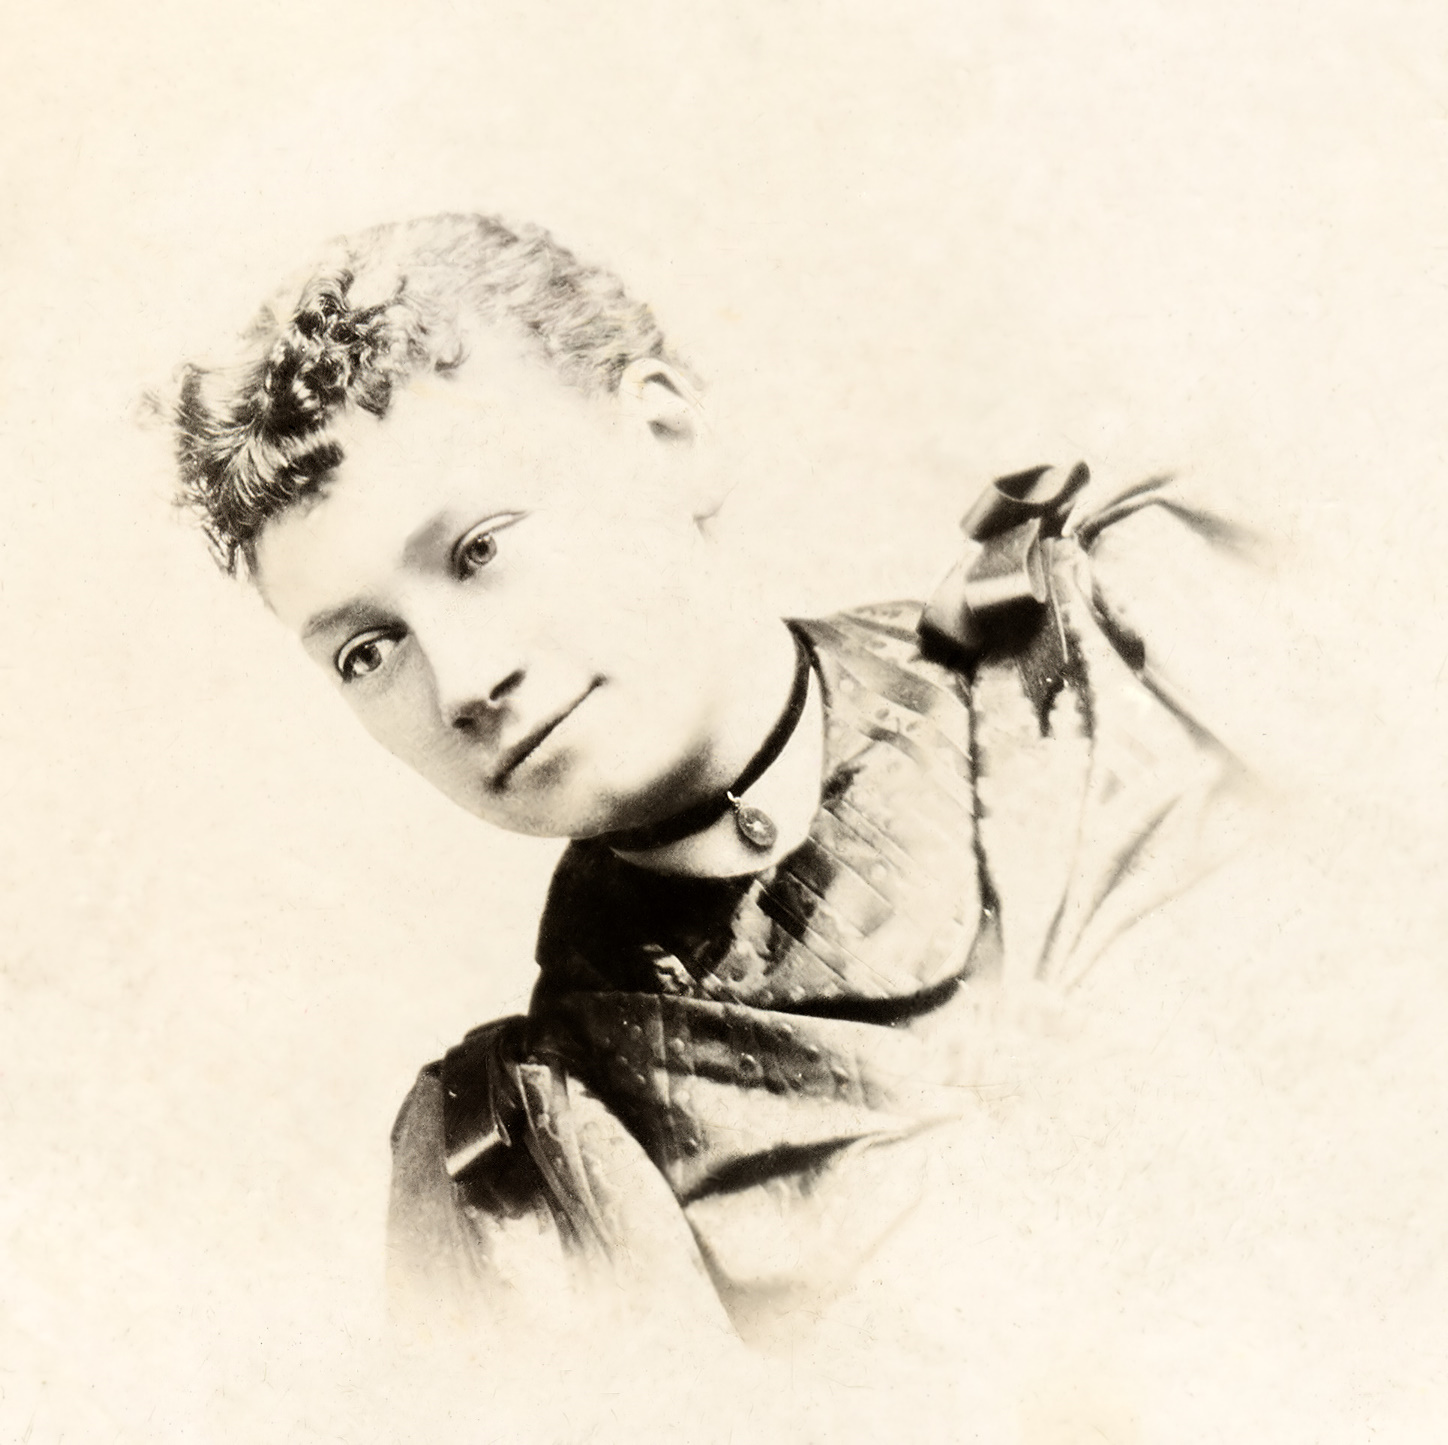
\includegraphics[width=0.23\textwidth]{dad-old-sweetheart.jpg}
%\caption{~~~IMCAPTION~~~}
%\label{fig:4230X3}
%\end{floatingfigure}
%\end{figure}

%\captionsetup[floatingfigure]{labelformat=empty}
%\begin{figure}[htbp]
%\begin{floatingfigure}[l]{0.25\textwidth}
%\centering
%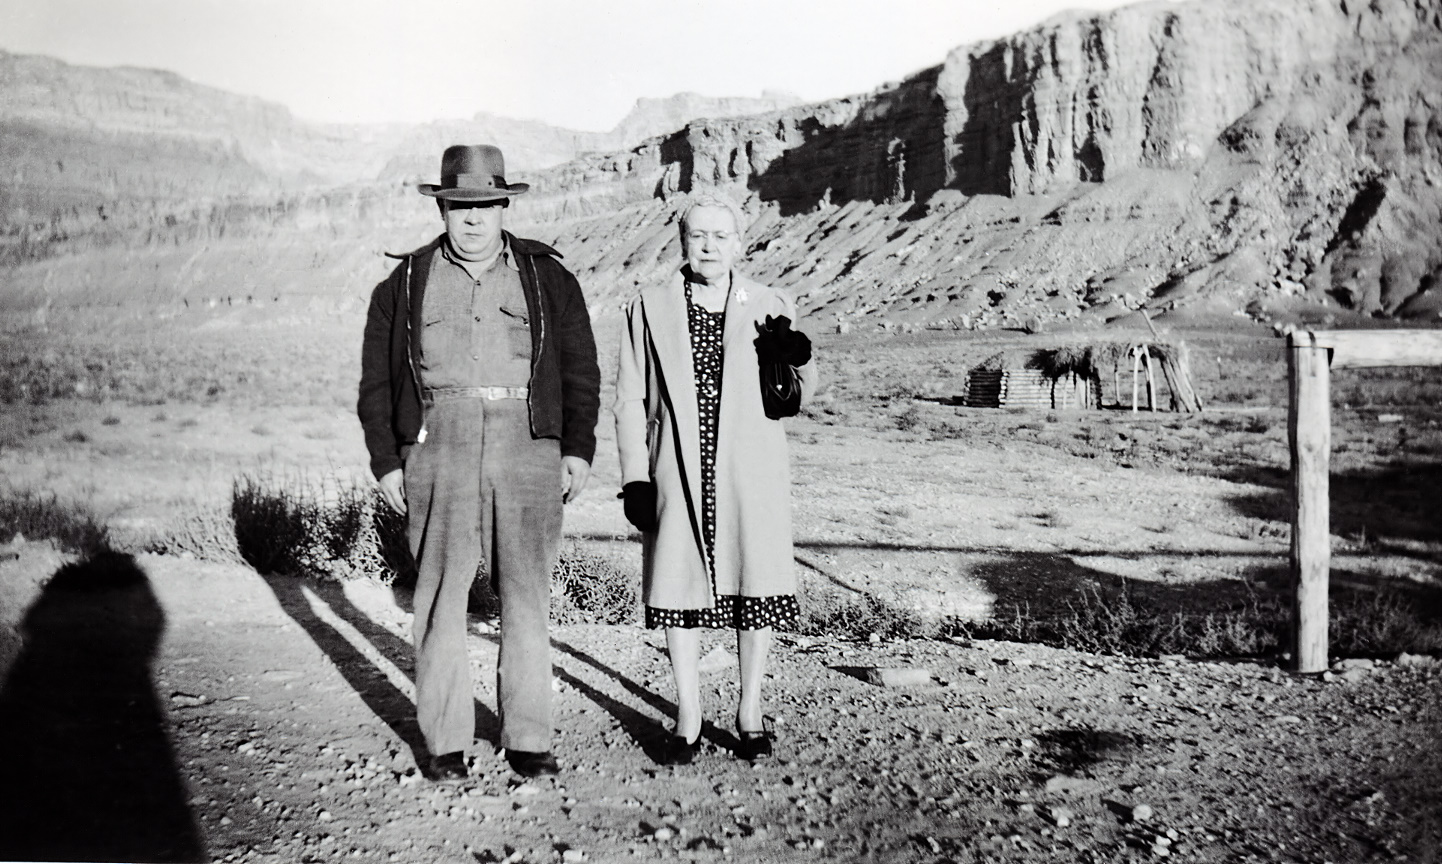
\includegraphics[width=0.23\textwidth]{vernon-minnie-raver-marble-canyon-arizona-1949.jpg}
%\caption{~~~IMCAPTION~~~}
%\label{fig:4230X4}
%\end{floatingfigure}
%\end{figure}

%\captionsetup[floatingfigure]{labelformat=empty}
%\begin{figure}[htbp]
%\begin{floatingfigure}[l]{0.25\textwidth}
%\centering
%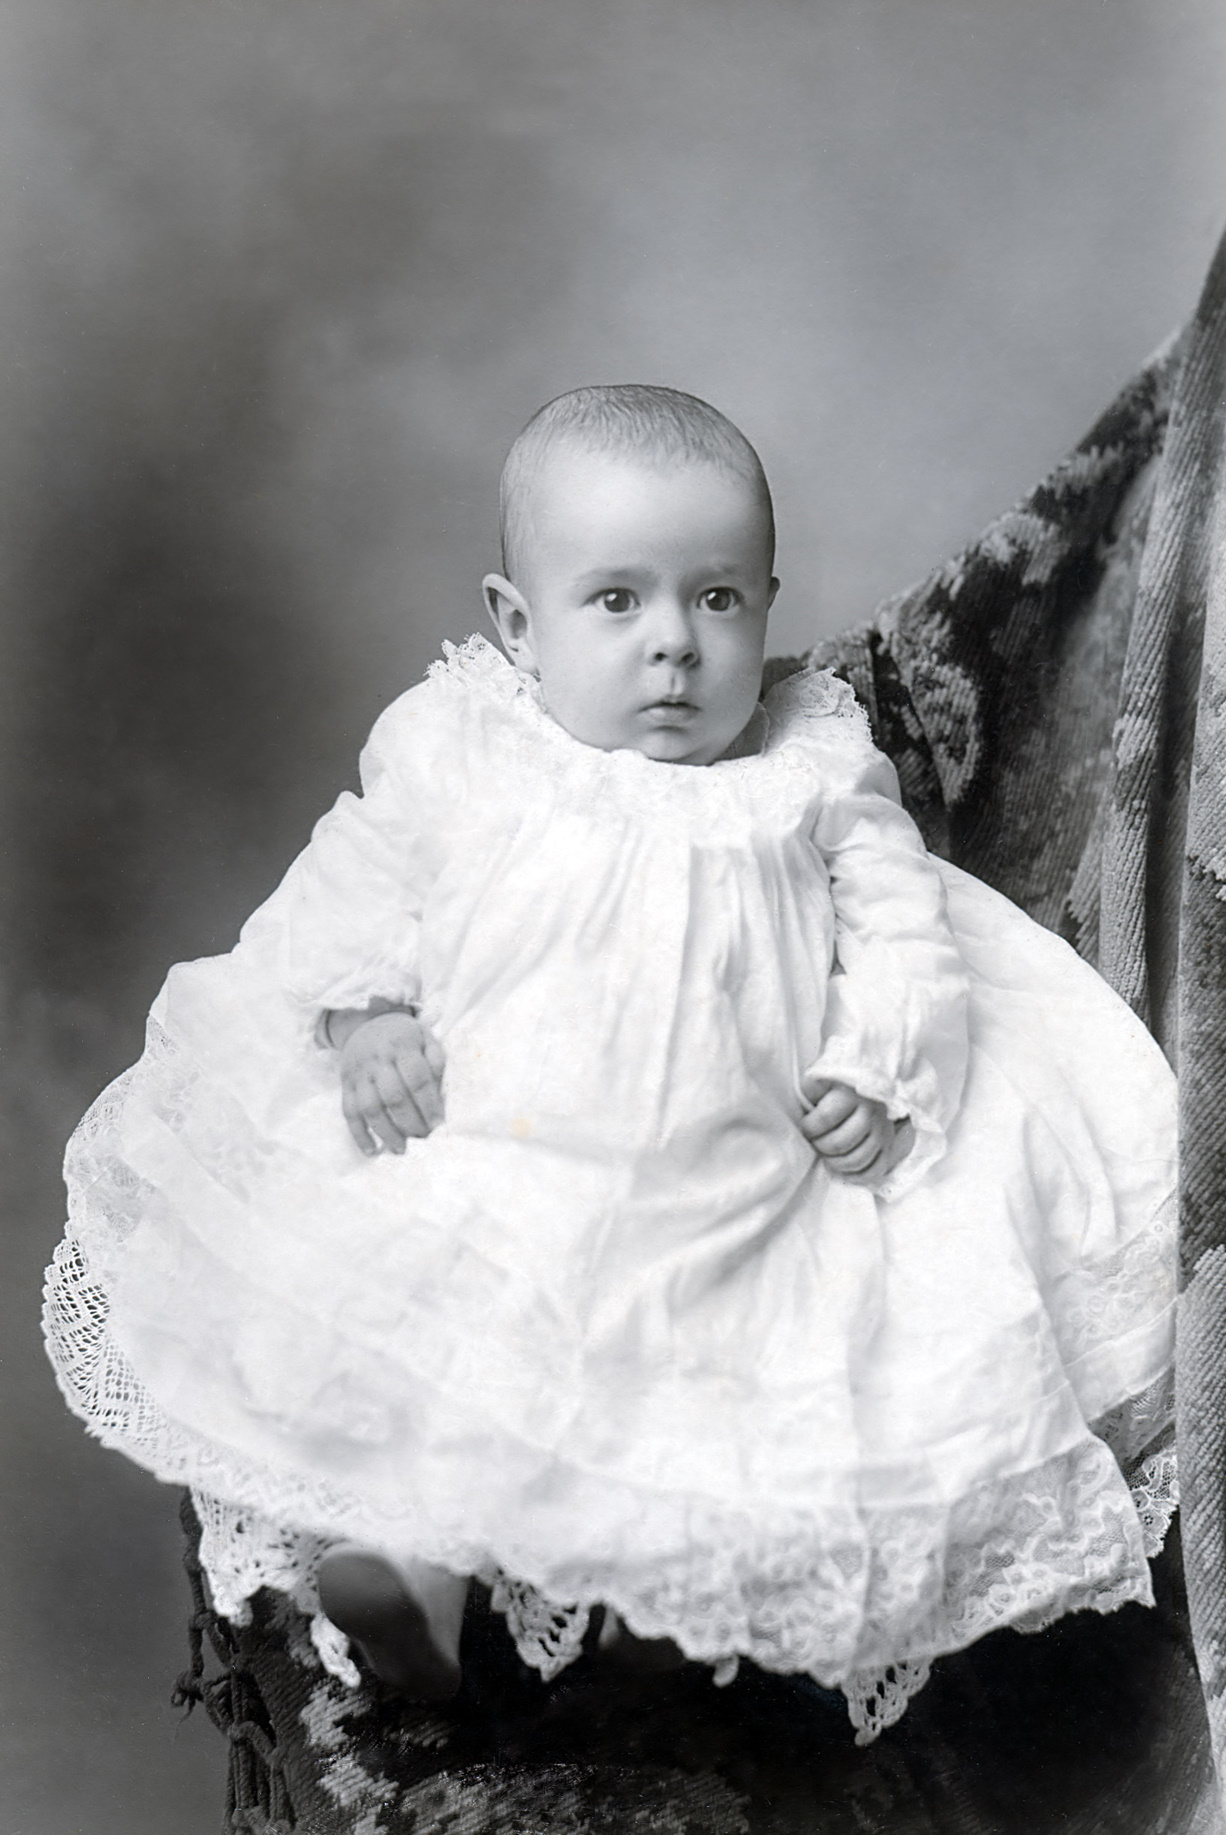
\includegraphics[width=0.23\textwidth]{vernon-raver-hazels-brother.jpg}
%\caption{~~~IMCAPTION~~~}
%\label{fig:4230X5}
%\end{floatingfigure}
%\end{figure}



%\end{document}